%&pdflatex
%%%%%%%%%%%%%%%%%%%%%%%%%%%%%%%%%%%%%%%%%%%%%%%%%%%%%%%%%%%%%%%%%%%%%%%%%%%%%%%%
%2345678901234567890123456789012345678901234567890123456789012345678901234567890
%        1         2         3         4         5         6         7         8

\documentclass[3p,onecolumn,authoryear]{elsarticle}  % Comment this line out if you need a4paper


% make changes take effect
\pagestyle{headings}
% adjust as needed
\addtolength{\footskip}{0\baselineskip}
\addtolength{\textheight}{-1\baselineskip}




%\documentclass[a4paper, 10pt, conference]{ieeeconf}      % Use this line for a4 paper

%\IEEEoverridecommandlockouts                              % This command is only needed if 
                                                          % you want to use the \thanks command

% See the \addtolength command later in the file to balance the column lengths
% on the last page of the document

% The following packages can be found on http:\\www.ctan.org
\usepackage{graphicx} % for pdf, bitmapped graphics files
\usepackage{epstopdf}
%\usepackage{epsfig} % for postscript graphics files
%\usepackage{mathptmx} % assumes new font selection scheme installed
%\usepackage{times} % assumes new font selection scheme installed
\let\proof\relax
\let\endproof\relax
\usepackage{amsmath} % assumes amsmath package installed
\usepackage{amsthm}  % For special theorem style
\usepackage{amsfonts}
%\usepackage{amssymb}  % assumes amsmath package installed
\usepackage[dvipsnames]{xcolor}
\usepackage{tikz}
\usepackage{pgfplots}
\usetikzlibrary{shapes,arrows}
\usetikzlibrary{backgrounds}
\usepackage{multirow}
\usepackage[keeplastbox]{flushend}
%\usepackage{cite}  % Make sure that citation appear as [1]-[3] instead of [1], [2], [3]
\usepackage[utf8]{inputenc}    % utf8 support
\usepackage[T1]{fontenc}       % code for pdf file
\usepackage[USenglish]{babel}             %% language support

\usepackage{url}
\usepackage{natbib}
\usepackage{letltxmacro}
\LetLtxMacro{\autocite}{\citep}
\LetLtxMacro{\textcite}{\citet}



\usepackage{pgfplots}
\pgfplotsset{compat=1.9}  % Prevent warning, pgf running in backwards compatibility mode anyway%\usetikzlibrary{external}                       %% Create pdf figures from TikZ. Use PDFTeXify ...
%\tikzexternalize[prefix=tikz/]                  %% ... with --tex-option=--shell-escape switch.
\usepackage[capitalize]{cleveref}
\Crefname{figure}{Fig.}{Figs.}
\crefname{equation}{}{}
\Crefname{equation}{Equation}{Equations}
\usepackage{subcaption}
\usepackage{xstring}
\usepackage{xparse}
\usepackage{siunitx}

\theoremstyle{plain}
\newtheorem{definition}{Definition}
\theoremstyle{remark}\newtheorem{remarkenv}{Remark}        %% remarks
\newenvironment{remark}{\begin{remarkenv}}%
	{\hfill$\lozenge$\end{remarkenv}}            %% end remark with a lozenge

%\pgfplotsset{compat=newest} 
%\pgfplotsset{plot coordinates/math parser=false}

%Images path 
\graphicspath{ {figures/} }


%\author{Erwin de Gelder$^{a,b*}$, Jan-Pieter Paardekooper$^{a,c}$, Arash Khabbaz Saberi$^{a}$, Hala Elrofai$^{a}$, Olaf Op den Camp$^{a}$, \\ Jeroen Ploeg$^{d,e}$, Ludwig Friedmann$^{f}$, Bart De Schutter$^{b}$%
%\thanks{$^{a}$TNO, P.O. Box 756, 5700 AT Helmond, The Netherlands}%
%\thanks{$^{b}$Delft University of Technology, Delft Center for Systems and Control, Delft, The Netherlands}%
%\thanks{$^{c}$Radboud University, Donders Institute for Brain, Cognition and Behaviour, Nijmegen, The Netherlands}%
%\thanks{$^{d}$2getthere, Utrecht, The Netherlands}%
%\thanks{$^{e}$Eindhoven University of Technology, Department of Mechanical Engineering Dynamics and Control group, Eindhoven, The Netherlands}%
%\thanks{$^{f}$BMW Group, Petuelring 130, 80788 Munich, Germany}%
%\thanks{$^{*}$Corresponding author. E-mail address: {\tt\small erwin.degelder@tno.nl}}%
%}

\author[1,2]{Erwin de Gelder\corref{cor1}}
\ead{erwin.degelder@tno.nl}
\author[1,3]{Jan-Pieter Paardekooper}
\author[1]{Arash Khabbaz Saberi}
\author[1]{Hala Elrofai}
\author[1]{Olaf Op den Camp}
\author[4,5]{Jeroen Ploeg}
\author[6]{Ludwig Friedmann}
\author[2]{Bart De Schutter}
\cortext[cor1]{Corresponding author, e-mail: \url{erwin.degelder@tno.nl}}
\address[1]{TNO, Dept.\ of Integrated Vehicle Safety, Helmond, The Netherlands}
\address[2]{Delft University of Technology, Delft Center for Systems and Control, Delft, The Netherlands}
\address[3]{Radboud University, Donders Institute for Brain, Cognition and Behaviour, Nijmegen, The Netherlands}
\address[4]{2getthere, Utrecht, The Netherlands}
\address[5]{Eindhoven University of Technology, Dept.\ of Mechanical Engineering Dynamics and Control group, Eindhoven, The Netherlands}
\address[6]{BMW Group, Petuelring 130, 80788 Munich, Germany}

\newlength\figurewidth
\newlength\figureheight
\newlength\venncircle
\newlength\objectwidth\setlength{\objectwidth}{18.5em}


\usetikzlibrary{arrows,positioning}
\usetikzlibrary{arrows.meta}
\definecolor{TNOlightgray}{RGB}{222,222,231}
\definecolor{scenariocategory}{RGB}{137, 197, 255}
\definecolor{category}{RGB}{121, 221, 255}
\definecolor{scenario}{RGB}{255, 157, 121}
\definecolor{otherclass}{RGB}{255, 188, 163}
\tikzstyle{tag}=[text height=.8em, text depth=.1em, font=\small\sffamily, rounded corners=0.2em, fill=TNOlightgray, node distance=9em, text width=7em, align=center]
\tikzstyle{tag wide}=[tag, text width=12em]
\tikzstyle{tagarrow}=[->, line width=0.75mm, color=TNOlightgray]
\tikzstyle{object}=[draw, text width=\objectwidth-.5em, align=left, line width=1pt, minimum width=\objectwidth, anchor=north west, node distance=3pt]
\newcounter{tagbcounter}
\newcounter{tagccounter}
\newcommand{\taga}[1]{
	\node[tag wide](taga){#1};
	\node[coordinate, below of=taga, node distance=1.2em](helper){};
}
\newcommand{\tagb}[3]{
	\node[tag, below of=taga, node distance=3em, xshift=#3](tagb#2){#1};
	\draw[tagarrow] (taga) -- (helper) -| (tagb#2);
	\node[coordinate, xshift=1em](tagb#2 helper) at (tagb#2.south west) {};
}
\newcommand{\tagc}[4]{
	\node[tag, below of=tagb#4, node distance=#3em, xshift=2em](tagc#2){#1};
	\draw[tagarrow] (tagb#4 helper) |- (tagc#2);
}
\ExplSyntaxOn
\NewDocumentCommand{\tree}{O{} m m}{%
	\begin{tikzpicture}
	\taga{#2}
	\setcounter{tagbcounter}{0}
	\seq_set_split:Nnn \arg { ; } { #3 }
	\seq_map_inline:Nn \arg {
		\seq_set_split:Nnn \argb {,} {##1}
		\seq_pop_left:NN \argb \argl
		\tagb{\argl}{\arabic{tagbcounter}}{\arabic{tagbcounter}*10em-\seq_count:N \arg *5em+5em}
		\setcounter{tagccounter}{0}
		\seq_map_inline:Nn \argb {
			\stepcounter{tagccounter}
			\tagc{####1}{\arabic{tagccounter}}{2*\arabic{tagccounter}}{\arabic{tagbcounter}}
		}
		\stepcounter{tagbcounter}
	}
	#1
	\end{tikzpicture}
}
\ExplSyntaxOff

% Notations
\newcommand{\amplitude}{\Delta v}
\newcommand{\attrtstart}{start time}
\newcommand{\attrtend}{end time}
\newcommand{\distancecondition}{d_{\mathrm{v,p}}}
\newcommand{\duration}{T}
\newcommand{\east}{x}
\newcommand{\north}{y}
\newcommand{\head}{\phi}
\newcommand{\egosub}{ego}
\newcommand{\egoeast}{\east_{\mathrm{\egosub}}}
\newcommand{\egonorth}{\north_{\mathrm{\egosub}}}
\newcommand{\egospeed}{\dot{\east}_{\mathrm{\egosub}}}
\newcommand{\egospeedinitsymbol}{v}
\newcommand{\egospeedinit}{\egospeedinitsymbol_{0}}
\newcommand{\egospeedinitb}{\egospeedinitsymbol_{0}}
\newcommand{\egospeedinitc}{\egospeedinitsymbol_{0}}
\newcommand{\egoacceleration}{\ddot{\east}_{\mathrm{\egosub}}}
\newcommand{\egoheading}{\head_{\mathrm{\egosub}}}
\newcommand{\function}{f}
\newcommand{\inputsystem}{u}
\newcommand{\dimensionstate}{n}
\newcommand{\parameter}{\theta}
\newcommand{\parametera}{a}
\newcommand{\parameterb}{b}
\newcommand{\pedsub}{ped}
\newcommand{\pedeast}{\east_{\mathrm{\pedsub}}}
\newcommand{\pednorth}{\north_{\mathrm{\pedsub}}}
\newcommand{\pednorthinit}{\north_{0}}
\newcommand{\pedheading}{\head_{\mathrm{\pedsub}}}
\newcommand{\pedspeed}{\dot{\north}_{\mathrm{\pedsub}}}
\newcommand{\origin}{O}
\newcommand{\scenario}{S}
\newcommand{\scenarioa}{\scenario_{1}}
\newcommand{\scenariob}{\scenario_{2}}
\newcommand{\scenarioc}{\scenario_{3}}
\newcommand{\comprises}{\ni}
\newcommand{\scenariocategory}{\mathcal{C}}
\newcommand{\scenariocategorya}{\scenariocategory_{1}}
\newcommand{\scenariocategoryb}{\scenariocategory_{2}}
\newcommand{\scenariocategoryc}{\scenariocategory_{3}}
\newcommand{\includes}{\supseteq}
\newcommand{\slopeego}{a_{\mathrm{\egosub}}}
\newcommand{\slopepedestrian}{v_{\mathrm{\pedsub}}}
\newcommand{\state}{x}
\newcommand{\statedot}{\dot{\state}}
\renewcommand{\time}{t}
\newcommand{\inittime}{\time_{0}}
\newcommand{\inittimeb}{\time_{1}}
\newcommand{\inittimec}{\time_{2}}
\newcommand{\hasone}{$1$}
\newcommand{\hasn}{$N$}

%\usepackage{changebar}
\newcommand{\cstart}{}  % Revision 2 changes (from 11 Jan 2019)
\newcommand{\cend}{}
%\newcommand{\todo}[1]{\color{red}TODO: #1\color{black}}

%\usepackage{setspace}
%\doublespacing


\begin{document}


%\thispagestyle{empty}
%\pagestyle{empty}
\title{Ontology for Scenarios for the Assessment of Automated Vehicles}


%%%%%%%%%%%%%%%%%%%%%%%%%%%%%%%%%%%%%%%%%%%%%%%%%%%%%%%%%%%%%%%%%%%%%%%%%%%%%%%%
\begin{abstract}
	% Explain issue: assessment is important
	
	The development of assessment methods for the performance of Automated Vehicles (AVs) is essential to enable and speed up the deployment of automated driving technologies, due to the complex operational domain of AVs.
	% Introduce scenarios (for assessment)
	As traditional methods for assessing vehicles are not applicable for AVs, other approaches have been proposed. 
	Among these, real-world scenario-based assessment is widely supported by many players in the automotive field. 
	In this approach, test cases are derived from real-world scenarios that are obtained from driving data.
	
	% Problem -> definition needed for scenario
	To minimize any ambiguity regarding these test cases and scenarios, a clear definition of the notion of scenario is required.
	% Solution: concrete definitions
	In this paper, we propose a more concrete definition of scenario, compared to what is known to the authors from the literature. This is achieved by proposing an ontology in which the quantitative building blocks of a scenario are defined.
	% Example
	An example illustrates that the presented ontology is applicable for scenario-based assessment of AVs.
\end{abstract}

\maketitle


%%%%%%%%%%%%%%%%%%%%%%%%%%%%%%%%%%%%%%%%%%%%%%%%%%%%%%%%%%%%%%%%%%%%%%%%%%%%%%%%
\section{Introduction}
\label{sec:introduction}

% Our contribution
An essential aspect in the development of automated vehicles (AVs) is the assessment of quality and performance aspects of the AVs, such as safety, comfort, and efficiency \autocite{bengler2014threedecades, stellet2015taxonomy, Helmer2017safety, putz2017pegasus, roesener2017comprehensive, gietelink2006development, wachenfeld2016release}.
For legal and public acceptance of AVs, a clear definition of system performance is important, as well as quantitative measures for system quality. 
Traditional methods, such as \autocite{response2006code, ISO26262}, used for the evaluation of driver assistance systems, are no longer sufficient for the assessment of quality and performance aspects of an AV, because they would require too many resources \autocite{wachenfeld2016release}. 
Therefore, among other methods, a scenario-based approach has been proposed \autocite{elrofai2018scenario, putz2017pegasus}. 
For scenario-based assessment, proper specification of scenarios is crucial since they are directly reflected in the test cases used for scenario-based assessment \autocite{stellet2015taxonomy}. 

% Explain importance/relevance
The notion of scenario is frequently used in the context of automated driving \autocite{putz2017pegasus, roesener2017comprehensive, gietelink2006development, hulshof2013autonomous, ebner2011identifying, ploeg2017GCDC, zofka2015datadrivetrafficscenarios, xiong2015orchestration, shao2019evaluating}, despite the fact that an explicit definition is often not provided. 
However, as mentioned by various authors \autocite{stellet2015taxonomy, Helmer2017safety, alvarez2017prospective, zofka2015datadrivetrafficscenarios, aparicio2013pre, putz2017pegasus, geyer2014, ulbrich2015}, using a scenario in the context of the development or assessment of AVs requires a clear definition of a scenario. 
To this end, some definitions of a scenario in the context of (automated) driving have been proposed in literature \autocite{geyer2014, ulbrich2015, elrofai2016scenario}.
These definitions, however, leave room for interpretation because, firstly, the definitions themselves are ambiguous and, secondly, the definitions use other undefined terms.
For the context of the assessment of AVs, scenarios are used to describe the test conditions \autocite{stellet2015taxonomy} and this requires a more concrete definition of a scenario to minimize any ambiguity.


% What is the added value of this paper w.r.t. other work
% - Easier to apply event/scenario mining, because more concrete
% - Important step towards quantification of completeness
% - More complete (also event defined etc.)
% - Backed up with literature (should we mention this???)
% - Real example given
We aim for a definition of a scenario that is, on the one hand, broadly consistent with existing definitions \autocite{geyer2014, ulbrich2015, elrofai2016scenario} while, on the other hand, more concrete, such that it is applicable for scenario mining \autocite{elrofai2016scenario} and scenario-based assessment \autocite{stellet2015taxonomy, deGelder2017assessment}. We propose a definition that is concrete enough to be used in quantitative analysis required for the assessment of AVs. This is achieved by defining quantitative building blocks of a scenario in the form of activities, actors, and the static environment. In addition, we introduce the concept of a \emph{scenario category}  
that is used to qualitatively describe scenarios, i.e., an abstraction of a scenario. 
\cstart To define the terms \emph{scenario} and \emph{scenario category}, we use terms that are commonly used in the field of the safety assessment of AVs \autocite{catapult2018musicc,catapult2018regulating,sigsim2019glossary,openscenario,ulbrich2015,geyer2014}. For an unambiguous formulation, some definitions from the field of control theory are adopted.\cend


Besides defining the notion of scenario, its building blocks, and the notion of scenario category, an ontology is presented that formalizes the description of a scenario and a scenario category. 
This ontology describes the relation between the different terms such as scenarios, activities, and actors.
Furthermore, the ontology enables the translation of the terms to object-oriented code.
This, in turn, is used to describe the scenarios in a coding language that can be understood by various software agents, such as simulation tools. The implementation code of our ontology is publicly available\footnote{As a coding language, Python is used. The code is publicly available at \url{https://github.com/ErwindeGelder/ScenarioDomainModel}.}. 
The ontology is also used as a schema for a database system for storing the scenarios and scenario categories.
An example is provided that illustrates the use of the ontology with a real-world case.

Ontologies have been widely used in the field of automated driving \autocite{provine2004ontology, morignot2013ontology, schlenoff2003using, zhao2015core, maiti2017conceptualization, benvenuti2017ontologybased, bagschik2017ontology}. However, to the best of our knowledge, we are the first to propose an ontology for scenarios for the assessment of AVs. 
From the implementation side, there are several file formats and methods for scenario ontologies, e.g., OpenSCENARIO \autocite{openscenario} and CommonRoad \autocite{althoff2017CommonRoad}. 
\cstart These implementations are used to describe specific tests for AVs that can be executed in a virtual environment.
Because of the focus on scenarios that can be simulated, these implementations describe scenarios at a quantitative level and, consequently, they do not provide concepts for a qualitative description of a scenario. \cend
Our proposed ontology differs from these implementations as our ontology also allows for qualitative descriptions of scenarios, which is useful because it enables to group scenarios and to interpret the scenarios more easily.
Furthermore, our ontology is supported with the definitions and justifications of each of the terms.

% Outline
The outline of the paper is as follows. In \cref{sec:background}, we explain why an ontology is useful, what the context is, and we provide some definitions of terms that are adopted from literature. 
Using these definitions and considering the context, we define the notions of \emph{scenario}, \emph{event}, \emph{activity}, and \emph{scenario category}  in \cref{sec:definitions}. 
The ontology that formalizes these definitions is presented in \cref{sec:ontology}. 
In \cref{sec:example}, an application example is provided to illustrate the use of the ontology with a real-world scenario. 
The paper is concluded in \cref{sec:conclusion}.


\section{Background}
\label{sec:background}

We first explain in \cref{sec:why ontology} why we want to present an ontology for describing scenarios and  scenario categories. Next, in \cref{sec:context}, we provide some information on the context for which we want to define scenarios. In \cref{sec:nomenclature}, we describe notions that are adopted from literature to define our ontology.



\subsection{Why an ontology?}
\label{sec:why ontology}
According to Gruber \autocite{gruber1993ontology}, ``an ontology is an explicit specification of a conceptualization'', where a conceptualization refers to ``an abstract, simplified view of the world that we wish to represent for some purpose''. Ontologies are widely applied in all kinds of research areas, e.g., computing \autocite{chen2004soupa}, vehicle platooning \autocite{maiti2017conceptualization}, system performance \autocite{benvenuti2017ontologybased}, transportation \autocite{katsumi2018ontologies}, and vehicle path planning \autocite{provine2004ontology, schlenoff2003using}. 
%Furthermore, ontologies are defined for various applications, e.g., for the profiling of users \autocite{golemati2007creating}, for the formalization of human activities \autocite{lee2017location}, and for product life cycle management \autocite{matsokis2010plm}. 
An ontology offers the following benefits:
\begin{itemize}
	\item An ontology is useful for sharing knowledge between people and software agents \autocite{vanDamPhDThesis2009, noy2001ontology}. For example, the ontology can be used for communication between different software agents, such as different simulation tools \autocite{shao2019evaluating}.
	\item An ontology can be directly translated into a class structure for an object-oriented software implementation \autocite{vanDamPhDThesis2009}. The ontology then specifies the relationships between the different classes and provides information on the properties of a class and the possible values.
	\item Domain assumptions about terms and definitions are made explicit \autocite{noy2001ontology}. 
	For example, we define the term \emph{scenario} in \cref{sec:scenario} and  this does not only help in preventing any ambiguity when communicating about scenarios, it also helps in understanding the underlying implementations, e.g., the programming language code, when assumptions are explicit.
	\item An ontology can be used as a conceptual schema in database systems  \autocite{gruber1993ontology}. A conceptual schema allows ``databases to interoperate without having to share data structures'' \autocite{gruber1993ontology}. In addition, a conceptual schema can be directly used to design the structure of a database.
\end{itemize}

There are several languages dedicated to the implementation of an ontology. Two major technologies are the Web Ontology Language (OWL)\footnote{OWL is the standard abbreviation for the Web Ontology Language.} and the Unified Modeling Language (UML). 
%We use UML for implementing the ontology, because UML focuses on describing implementation related issues, which is useful considering our Python implementation.
For a detailed comparison between OWL and UML, we refer the interested reader to \autocite{kiko2005detailed}.



\subsection{Context of a scenario}
\label{sec:context}

Because the notion of scenario is used in many different contexts, a wide diversity in definitions of this notion exists (for an overview, see \autocite{vannotten2003updated, bishop2007scentechniques}). Therefore, it is reasonable to assume that ``there is no [generally] `correct' scenario definition'' \autocite{vannotten2003updated}. As a result, to define the notion of scenario, it is important to consider the context in which it will be used. 

In this paper, the context of a scenario is the assessment of AVs, where AVs refer to vehicles equipped with a driving automation system\footnote{According to \autocite{sae2018j3016}, a driving automation system is ``the hardware and software that are collectively capable of performing part or all of the dynamic driving task on a sustained basis. This term is used generically to describe any system capable of level 1-5 driving automation.'' Here, level 1 driving automation refers to ``driver assistance'' and level 5 refers to ``full driving automation''. For more details, see \autocite{sae2018j3016}.}. 
It is assumed that the assessment methodology uses scenarios. %(i.e., test cases) 
%for which some resulting metrics are compared with a reference \autocite{stellet2015taxonomy}. 
% - Scenarios that an (automated) vehicle can encounter
The ultimate goal is to build a database with all relevant scenarios that an AV has to cope with when driving in the real world \autocite{putz2017pegasus}. Hence, a scenario should be a description of a potential use case of an AV. 
% Whether these scenarios are obtained with a knowledge-based approach \autocite{gietelink2004systemvalidation, stellet2015taxonomy} or with a data-driven approach \autocite{deGelder2017assessment, stellet2015taxonomy}, a clear and unambiguous definition of such a test scenario is required. 

%In this paper, \emph{scenario} can refer to either an observed scenario in (real-world driving) data, i.e., a real-world scenario, or a scenario that is used for testing AVs, i.e., a test case. Note that, typically, the difference between the two is that with a real-world scenario, the activity of all actors is described, while for a test case, some goals are specified for the system under test (e.g., the goal could be to drive from A to B) instead of its activity. 



\subsection{Nomenclature}
\label{sec:nomenclature}
For the definition of \emph{scenario}, several notions are adopted from literature. In this section, the concepts of \emph{ego vehicle}, \emph{actor}, \emph{state variable}, \emph{state vector}, \emph{model}, \emph{mode}, \emph{act}, \emph{static environment}, and \emph{dynamic environment} are detailed. 

\subsubsection{Ego vehicle}
\label{sec:ego vehicle}
The ego vehicle refers to the perspective from which the world is seen. In particular, the ego vehicle refers to the vehicle that is perceiving the world through its sensors (e.g., see \autocite{Bonnin2014}). When performing tests, the ego vehicle also refers to the vehicle that must perform a specific task (e.g., see \autocite{althoff2017CommonRoad}). In this case, the ego vehicle is often referred to as the system under test \autocite{stellet2015taxonomy}, the vehicle under test \autocite{gietelink2006development}, or the host vehicle \autocite{gietelink2006development}.
%The ontology presented by Geyer~et~al.\ ``is described from the ego-vehicle's point of view'' \autocite{geyer2014}. 
%Note that in case a sensor-equipped vehicle is used to extract scenarios from real-world driving, the ego vehicle in an extracted scenario does not necessarily have to correspond to the sensor-equipped vehicle that is used to acquire the real-world data.

\subsubsection{Actor}
\label{sec:actor}

According to \textcite{catapult2018musicc}, ``actors are all dynamic components of a scenario, excluding the ego vehicle itself.'' In practice, this can be, for example, a driver of a car, a cyclist, a pedestrian, a driving automation system, or a combination of a driver and a driving automation system \autocite{geyer2014}. Note that, in contrast to \autocite{catapult2018musicc}, in the current paper, the ego vehicle's driver, and/or automation system are considered as actors, similar to \autocite{geyer2014},  because they have the same properties as another driver or automation system.

%: ``in this case, [the actor is] the ego-vehicle with driver/automation.''
%An actor is an element of a scenario acting on its own behalf \autocite{ulbrich2015}. 
% Traffic light?

\subsubsection{State variable} 
\label{sec:state variable}
\textcite[p.~163]{dorf2011modern} write that ``the state variables describe the present configuration of a system and can be used to determine the future response, given the excitation inputs and the equations describing the dynamics.'' In our case, ``the system'' could refer to an actor, a component, or a simulation. E.g., a state variable could be the acceleration of an actor.

\subsubsection{State vector}
\label{sec:state vector}
A state vector refers to ``the vector containing all $n$ state variables'' \autocite[p.~233]{dorf2011modern}.

\subsubsection{Model}
\label{sec:model}
Typically, a dynamical system is modeled using a differential equation of the form $\statedot(\time)=\function_{\parameter}(\state(\time), \inputsystem(\time), \time)$ \autocite{norman2011control}, where $\state(\time)$ represents the state vector at time $\time$, $\inputsystem(\time)$ represents an external input vector, and the function $\function_{\parameter}(\cdot)$ is parameterized by $\parameter$.  Note that, technically speaking, $\state(\cdot)$, $\inputsystem(\cdot)$, $\time$, and $\parameter$ are inputs of the function $\function$, but $\parameter$ is assumed to be constant for a certain time interval. For example, the following first-order model is parameterized by $\parameter=(\parametera,\parameterb)$:
\begin{equation}
\statedot(\time) = \parametera \state(\time) + \parameterb \inputsystem(\time).
\end{equation}

% The input $u$ is a function of time, that needs to be quantified. For this purpose, a parametrized function can be used, i.e. $u=g_{\theta}(t)$ with parameter vector $\theta$, such that the differential equation can be rewritten to $\dot{x}=h_{\theta}(x,t)$. In the context of this paper, model refers to a parametrized function, such as $h_{\theta}(x,t)$. It might be more practical to directly model the state (i.e., the result of the differential equation) using a function $x=k_{\theta}(t)$, such that no explicit information is required about the system dynamics. For example, see \autocite{deGelder2017assessment}.

\subsubsection{Mode}
\label{sec:mode}
In some systems, the behavior of the system may suddenly change abruptly, e.g., due to a sudden change in an input, a model parameter, or the model function. Such a transition is called a mode switch.
In each mode, the behavior of the system is described by a model with a fixed function $f_{\theta}$ and smooth input $u(\cdot)$ \autocite{deschutter2000optimal}.

%\subsubsection{Activity}
%\label{sec:activity}
%An activity refers to the behavior of a particular mode. For example, an activity could be described by the label `braking' or `changing lane'.
%A scenario contains the quantitative description of the ongoing activity of the ego vehicle and its dynamic environment. Here, the description refers to the changing states that are relevant for the scenario, e.g., acceleration and velocity. The activity is described using the models that describe the way the state evolves over time.


\subsubsection{Act}
\label{sec:act}

We define act as the combination of actors and the activities that are performed by the actors. %Additionally, the act can contain conditions that mark the start or end of the act.
This is in accordance with the use of the term \emph{act} in \autocite{openscenario}. 


\subsubsection{Static environment}
\label{sec:static environment}
The static environment refers to the part of the environment that does not change during a scenario. This includes geo-spatially stationary elements \autocite{ulbrich2015},  such as the road network.
%Although one might argue whether light and weather conditions are dynamic or not \autocite{geyer2014,bach2016modelbased}, in most cases it is reasonable to assume that these conditions are not subject to significant changes during the time frame of a scenario. 
%Hence, light and weather conditions are usually part of the static environment.

\subsubsection{Dynamic environment}
\label{sec:dynamic environment}
As opposed to the static environment, the dynamic environment refers to the part of a scenario that changes during the time frame of a scenario. 
%The dynamic environment is described using the activities that describe the way the states evolve over time. 
In practice, the dynamic environment mainly consists of the moving actors (other than the ego vehicle) that are relevant to the ego vehicle.
For example, the primary use case of OpenSCENARIO, a file format for the description of the dynamic content of driving simulations, is to describe ``complex, synchronized maneuvers that involve multiple entities like vehicles, pedestrians, and other traffic participants'' \autocite{openscenario}, so for OpenSCENARIO, these maneuvers represent the dynamic environment.
Roadside units that communicate with vehicles within the communication range \autocite{alsultan2014comprehensive} are also part of the dynamic environment. Furthermore, changing (weather) conditions are part of the dynamic environment.

\begin{remark}
	Note that it might not always be obvious whether an element of the environment belongs to the static or dynamic environment. 
	%For example, the post of a traffic light can be considered as part of the static environment, while the signal of the traffic light can be considered as part of the dynamic environment.
	Most important, however, is that all parts of the environment that are relevant to the assessment of an AV are described in either the static or the dynamic environment.
\end{remark}


\section{Definitions}
\label{sec:definitions}

One of the main reasons to introduce an ontology is to enable sharing of knowledge between researchers, developers, and users. 
Therefore, it is important that the terms we use are clearly defined. 
When presenting our ontology in \cref{sec:ontology}, we will formalize the terms such that they can be used by software agents.
In this section, we will define the terms linguistically, thereby providing insight into the terms used in the next section.
We will first define the concept of a scenario in \cref{sec:scenario}. 
Next, we will define two important attributes of a scenario: events and activities, in \cref{sec:event,sec:activity}, respectively. 
Lastly, we will present the definition of a scenario category in \cref{sec:scenario category}.


In each of the \cref{sec:scenario,sec:event,sec:activity,sec:scenario category}, we start with background information. Next, we draw conclusions that lead to our proposed definition of the corresponding terms. After proposing a definition, we finish each section with remarks and implications of our proposed definition.




\subsection{Scenario}
\label{sec:scenario}

% Definition according to Go and Carroll
\textcite{go2004blind} describe a scenario within the field of system design. They define a scenario as ``a description that contains (1) actors, (2) background information on the actors and assumptions about their environment, (3) actors' goals or objectives, and (4) sequences of actions and events. Some applications may omit one of the elements or they may simply or implicitly express it. Although, in general, the elements of scenarios are the same in any field, the use of scenarios is quite different.'' 

% Definition according to Geyer et al.
\textcite{geyer2014} describe a scenario within the context of automated driving. They use the metaphor of a movie or a storybook for describing a scenario. \textcite{geyer2014} state that ``a scenario includes at least one situation within a scene including the scenery and dynamic elements. However, [a] scenario further includes the ongoing activity of one or both actors.'' For a further explanation of the terms situation, scene, and scenery, see \autocite{geyer2014}. 
%It is mentioned that the action of the driver and/or automation might be predefined. 
In \autocite{geyer2014}, the meaning of activity is not detailed.
%In an example of a so-called crossway scenario, they mention that the course of events might be different. For example, when a car keeps constant speed and then turns right, the scenario consists of one situation. The car might also first decelerate, accelerate and decelerate before turning right. In this case, the scenario consists of four situations.

% Definition according to Ulbrich et al.
\textcite{ulbrich2015} also define a scenario in the context of automated driving. They define a scenario as ``the temporal development between several scenes in a sequence of scenes. Every scenario starts with an initial scene. Actions \& events as well as goals \& values may be specified to characterize this temporal development in a scenario. Other than a scene, a scenario spans a certain amount of time.'' The authors of \autocite{ulbrich2015} state that actions and events link the different scenes. A further description of actions and events is not given in \autocite{ulbrich2015}.

% Definition according to Elrofai et al.
Another definition of a scenario in the context of automated driving is given by \textcite{elrofai2016scenario}. They define a scenario as ``the combination of actions and maneuvers of the host vehicle in the passive [i.e., static] environment, and the ongoing activities and maneuvers of the immediate surrounding active [i.e., dynamic] environment for a certain period of time.'' They further mention that the duration of a scenario typically is in the order of seconds.

% What is missing in the definitions?
% 1. No difference between qualitative and quantitative. I.e., definitions are ambiguous.
% 2. There are undefined terms.
% 3. Definitions are not detailed enough to reflect into code.

Although the aforementioned definitions of scenario \autocite{geyer2014, ulbrich2015, elrofai2016scenario} are in the context of automated driving, we require a more concrete definition. First, the aforementioned definitions do not specify the level of detail. 
%We experience much confusion where one group thinks a discussion is about a very specific scenario whereas another group thinks the same discussion is about a collection of scenarios that share some characteristics. 
Secondly, the aforementioned definitions use undefined terms, such as ``action'' and ``event''. Thirdly, because scenarios are used to specify test cases for the assessment of AVs, a clear and unambiguous specification of these scenarios is important and the aforementioned definitions are not concrete enough to be directly reflected into a coding language.



% "Requirements"
Before providing the definition of the notion of scenario, characteristics of the notion of scenario based on literature are listed as follows:
%
% Order of seconds
\begin{enumerate}
	\item \textit{A scenario corresponds to a time interval:}
	The aforementioned definitions \autocite{go2004blind, geyer2014, ulbrich2015, elrofai2016scenario} state that a scenario corresponds to a time interval. \textcite{vannotten2003updated} call such a scenario a chain scenario (``like movies''), as opposed to a snapshot scenario, i.e., a scenario that describes the state at a time instant (``like photos''). %The duration of a scenario is in the order of seconds, as explicitly mentioned by \textcite{elrofai2016scenario}. Though the duration is not mentioned by \textcite{ulbrich2015}, the presented example is in the order of seconds. Furthermore, other scenarios regarding (automated) driving are also in the order of seconds, e.g., see \autocite{gietelink2006development, zofka2015datadrivetrafficscenarios, roesener2017comprehensive, karaduman2013interactivebehavior, hulshof2013autonomous, englund2016grand}.
	
	% Scenarios consists of one or several events
	\item \textit{A scenario consists of one or several events \autocite{vannotten2003updated, go2004blind, geyer2014, ulbrich2015, kahn1962}:}
	It can be helpful to develop scenarios using events \autocite{bishop2007scentechniques}. Thus, a scenario could be defined as a particular sequence of events or, as \textcite[p.~143]{kahn1962} writes, ``a scenario results from an attempt to describe in more or less detail some hypothetical sequence of events''. Furthermore, \textcite{geyer2014} and \textcite{ulbrich2015} use the notion of event for describing a scenario, although they do not provide a definition of the term \emph{event}. In \cref{sec:event}, we will elaborate on the notion of \emph{event}.
	
	% Semantically described
	\item \textit{Real-world traffic scenarios are quantitative scenarios:}
	Regarding the nature of the data, a scenario can be either qualitative or quantitative \autocite{vannotten2003updated}. Real-world traffic scenarios are quantitative scenarios, such that they are, e.g., suitable for simulation purposes. A scenario, however, can also be described qualitatively, such that it is readable and understandable for human experts. Providing a qualitative description of a quantitative scenario has become known as a story-and-simulation approach \autocite{alcamo2001scenarios}. 
	Note that several quantitative scenarios might have the same qualitative description; thus, a qualitative description of a scenario does not uniquely define a quantitative scenario. A qualitative description can be regarded as an abstraction of the quantitative scenario, see also \cref{sec:scenario category}.
	
	% Some relevance between events
	\item\textit{The time interval of a scenario contains all relevant events:}
	According to \textcite{geyer2014}, ``the end of a scenario is defined by the first irrelevant situation with respect to the scenario''. In a similar manner, we require that the time interval of a scenario should contain all relevant events. Note that `relevant' is subjective and, therefore, an event is considered to be relevant, if it is relevant to the ego vehicle.
	% Next to that, an event is regarded as irrelevant, if it is independent of the relevant events.
	
	% Description of static environment
	\item\textit{A scenario includes the description of the environment:}
	A scenario should include the description of the static and dynamic environment.
	Although the description of the static environment is not a general prerequisite of a scenario, this is often included when speaking about traffic scenarios \autocite{geyer2014, ulbrich2015, elrofai2016scenario, ebner2011identifying, althoff2017CommonRoad}.
	%The static environment does not change during a scenario.
	The description of the dynamic environment includes a description of the type of actors and the goals and/or activities of the actors.
	
	%Everything that changes during the time interval of a scenario is considered to be part of the dynamic environment. 
	
	% Goals (instead of activities)
	\item\textit{A scenario describes the goals or activities of the ego vehicle:}
	For describing a scenario in real-world data, it is not necessary to describe the goals and therefore, \textcite{elrofai2016scenario} mention the activities of the ego vehicle rather than its goals. When describing a scenario that an AV has to cope with, however, its goals (i.e., its driving mission \autocite{geyer2014}) could be specified rather than its activities \autocite{ulbrich2015}. Note that if the activities of the ego vehicle are described rather than its goals, an observer might not be able to determine whether the ego vehicle has successfully responded to the scenario.
\end{enumerate}


% Definition
Hence, we define a scenario as follows:
\begin{definition}[Scenario]\label{def:scenario}
	A scenario is a quantitative description of the relevant characteristics of the ego vehicle, its activities and/or goals, its static environment, and its dynamic environment. In addition, a scenario contains all events that are relevant to the ego vehicle.
\end{definition}

% Describe difference from literature
% - quantitative --> to avoid ambiguous situation and to serve assessment
% - notion of scene not used. Scene follows from description, but is not explicitely used
%\Cref{def:scenario} deviates from existing definitions \autocite{geyer2014, ulbrich2015, elrofai2016scenario} in that it explicitly mentions that a scenario is quantitative. We use the term \emph{scenario class} to refer to the qualitative description, see \cref{sec:scenario class}.

\textcite{geyer2014} and \textcite{ulbrich2015} use the term \emph{scene} to define a scenario, while \cref{def:scenario} describes the scenes implicitly. Thus, the scenes do not have to be described explicitly.

%\Cref{fig:scenario} shows a schematic overview of the various components of a scenario. As shown in the second row of \cref{fig:scenario}, a scenario contains an ego vehicle, a dynamic environment, and a static environment. As an example, possible activities of the vehicle in front, which is part of the dynamic environment, are detailed by considering the state variables `heading' and `speed'. Note that a definition of the term activity is given in \cref{sec:activity}. The two rows of the activities show more generic descriptions and more detailed descriptions, respectively, of some possible activities.

%\begin{figure}
%	\centering
%	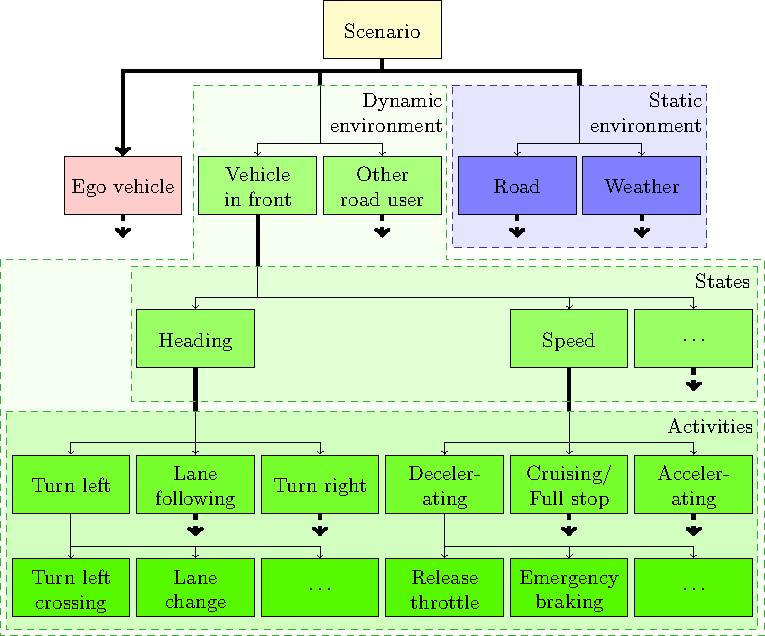
\includegraphics[width=0.5\linewidth]{figures/scenario.pdf}%
%	\caption{Schematic overview of a scenario. Note that the dynamic environment is not limited to the `vehicle in front', nor does it need to have the `vehicle in front'. Similarly, the static environment is not limited to `road', nor does it need to have `road'.}
%	\label{fig:scenario}
%\end{figure}


According to \cref{def:scenario}, a scenario describes, among others, the static environment. 
When it comes to applying this definition in an ontology, it is possible that ``describing'' the static environment is done by simply providing a reference to a static environment. 
This also holds for the other parts of a scenario. 
A reference could be, for example, the full name of a file, a pointer pointing to a specific part of the computer memory, or an identifier that addresses a specific entry in a database.
The advantage of references is that these parts of the scenario can be exchanged across different scenarios, as these scenarios can use the same references. 
As an example, an OpenSCENARIO file allows to provide a reference to an OpenDRIVE file which describes a road network \autocite{dupuis2010opendrive}. As we will see in \cref{sec:ontology}, in our proposed ontology, a scenario may contain references to a static environment, activities, actors, and events.




\subsection{Event}
\label{sec:event}
% Introduction of this section
As mentioned in \cref{def:scenario}, a scenario consists of events. 
%The notion of event is extensively used in literature \autocite{breu1997towards, pfeiffer2013concepts, branicky1998hybridcontrol, deschutter2000optimal, heemels2012eventcontrol}. In this section, a selected number of descriptions is presented. Next, a definition of event is given that suits our context.
% Literature review
The term event is used in many different fields, e.g.:
\begin{itemize}
	\item In computing \autocite{breu1997towards}, an event is an action or occurrence recognized by software. A common source of events are inputs by the software users. An event may trigger a state transition.
	%\item \textcite{kim1993supervenience}, a philosopher, writes: ``The term event ordinarily implies change''. \textcite{kim1993supervenience} states that an event is composed of three elements: objects, a property, and a time instant or a temporal interval. 
	\item In probability theory, an event is an outcome or a set of outcomes of an experiment \autocite{pfeiffer2013concepts}. For example, a thrown coin landing on its tail is an event.
	%\item ``In relativity, an event is any occurrence with which a definite time and a definite location are associated; it is an idealization in the sense that any actual event is bound to have a finite extent both in time and in space'' \autocite{sartori1996understanding}.
	\item In the field of hybrid systems theory, ``the continuous and discrete dynamics interact at `event' or `trigger' times when the continuous state [vector] hits certain prescribed sets in the continuous state space'' \autocite{branicky1998hybridcontrol}. ``A hybrid system can be in one of several modes, [...], and the system switches from one mode to another due to the occurrence of events'' \autocite{deschutter2000optimal}.
	\item In event-based control, a control action is computed when an event is triggered, as opposed to the more traditional approach where a control action is periodically computed \autocite{heemels2012eventcontrol}. In event-based control, the event is triggered at the moment at which the system (is about to) reach a certain threshold.
\end{itemize}

Before providing the definition of an event, the following is concluded about an event, based on aforementioned literature:

% It is a time instant
\begin{enumerate}
	\item\textit{An event corresponds to a time instant:}
	\cstart For the definition of event, we consider a hybrid-systems setting with a linear time model \autocite{alur1994theory}. Therefore, an event happens at some time instant.\cend
	
	% Event should mark transition of a state from one set to another - mention relation with hybrid control
	\item\textit{An event marks a mode transition or the moment a system reaches a threshold:} A mode transition may be \cstart induced \cend by either an abrupt change of an input signal, a change of a parameter, a change in the model, \cstart or an external cause. \cend It is also possible that the event marks the moment that a system reaches a threshold.
	
	%\item\textit{An event marks (a cause of) a mode transition}
	%Events mark the transition of mode, which is either a change of input, parameter or state. This is analogous to the way event is described in hybrid control \autocite{boel1999hybridcontrol}.
\end{enumerate}

% Give definition
Hence, we define an event as follows:
\begin{definition}[Event] \label{def:event}
	An event marks \cstart the moment a mode transition occurs or the moment a system reaches a specified threshold, where the former can be induced by both internal and external causes. \cend Before and after an event, the state vector of the system corresponds to two different modes.
\end{definition}

% Mention that there are basically two definitions. First definition more suitable for triggers for test cases. Second definition more suitable for observations and inputs.
Definition~2 indicates that the moment of an event can be defined in two different ways: \cstart(1) by a mode transition or (2) by the system reaching a threshold. 
The first type of event, i.e., a mode transition can occur at the moment of a sudden driver input. Furthermore, an event might also be induced by an external cause, such as an environmental change. The second type of event, i.e., related to the system reaching a threshold, \cend is especially useful when describing test cases. For example, consider the ego vehicle approaching a pedestrian that is about to cross the road \autocite{seiniger2015test}. 
Here, the event marks the moment that the distance between the vehicle and pedestrian is less than $\distancecondition$ meters. 
At the moment of this event, the pedestrian starts to cross the road such that the vehicle impacts the pedestrian if it does not change its speed or direction \autocite{seiniger2015test}.
By using a variable threshold $\distancecondition$, the value is flexible and can be set differently to define multiple scenarios.

For the practical implementation of events, a set of conditions may be specified. In that case, the event occurs at the moment that the conditions are met. A condition could be on, e.g., the distance between the vehicle and pedestrian. In \autocite{openscenario}, an extensive list of possible conditions that can be used to define an event is given.


%This first type of event, i.e., at the moment at which the system reaches a threshold, is related to events in event-based control \autocite{heemels2012eventcontrol}, whereas the second type of event, i.e., at the moment at which a mode transition occurs, is related to events in hybrid theory \autocite{deschutter2000optimal}. 
%Especially when designing scenarios for testing purposes, an event of the first type might trigger an event of the second type. For example, consider a vehicle approaching a zebra crossing with a pedestrian (dummy) that is about to cross the road at the zebra crossing. When the distance between the vehicle and the zebra crossing becomes less than 20 meters (event of the first type), the pedestrian (dummy) starts crossing the road at the zebra crossing (event of the second type).


%The inter-event time interval, i.e., the time in between two events, corresponds to a certain activity. For example, when the longitudinal acceleration is negative during an inter-event time interval, the activity can be described by the label `braking'.
%Another example of an event is the time instant at which the head lights are turned on. In that case, the activities before and after the event can be described as `lights off' and `lights on', respectively.



\subsection{Activity}
\label{sec:activity}

As mentioned in \cref{def:scenario}, a scenario  includes  a description of the dynamic environment of the ego vehicle. To describe the dynamic environment, activities are used. Furthermore, a scenario may describe the activities of the ego vehicle. 
% [Following sentence removed, because too obvious]
% Therefore, next to events, activities can be seen as the building blocks of a scenario.

Both the terms activity \autocite{geyer2014, elrofai2018scenario, childress2015using, catapult2018musicc, sigsim2019glossary} and action \autocite{geyer2014, ulbrich2015, bagschik2017ontology} are used in the context of automated driving. Although, strictly speaking, the terms action and activity have a slightly different meaning, they are often used for the same purpose:
\begin{itemize}
	\item According to \textcite{ulbrich2015}, actions may be specified for characterizing the temporal development in a scenario.
	\item \textcite{elrofai2018scenario} consider an activity as a building block of the dynamic part of the scenario: ``An activity is a time evolution of state variables such as speed and heading to describe for instance a lane change, or a braking-to-standstill.''
	\item In a glossary for a scenario catalog development \autocite{catapult2018musicc}, an activity is defined as ``the state [vector] of an object over an interval of time. An activity starts with an event and ends with another event.''
	%	\item According to the Cambridge Dictionary, an activity is defined as ``the doing of something, or something that you are doing, have done, or could do'' \autocite{cambridge2019activity}.
	%	\item \textcite{caspersen1985physical} define physical activity ``as any bodily movement produced by skeletal muscles that result in energy expenditure''.
	%	\item \textcite{bobick1997movement} simply states that an activity is a ``sequence of movements''. 
\end{itemize}


Before providing the definition of an activity, the following is concluded about an activity based on the aforementioned literature:

\begin{enumerate}
	% Time interval
	\item\textit{An activity corresponds to an inter-event time interval:}
	As opposed to an event, an activity spans over a certain time interval. Furthermore, the start and the end of an activity are marked by an event.
	
	% Describing the evolution of a state
	
	\item\textit{An activity quantitatively describes the time evolution of a state variable:}
	Because activities are building blocks of a scenario and a scenario corresponds to a quantitative description, the activities themselves need to be quantitative as well. 
	Therefore, an activity describes the time evolution of one or more state variables, i.e., the trajectory of one or more state variables over an inter-event time interval that corresponds to the activity, where the term state variable is defined in \cref{sec:state variable}.
	
	% Performed by something (an actor?)
	\item\textit{An activity is performed by an actor:}
	An activity quantitatively describes the time evolution of one or more state variables and a state variable corresponds to an actor, e.g., the acceleration of a vehicle, and, therefore, an activity is performed by an actor. Note that the actor might be the ego vehicle. 
	%However, it might also be the case that a state does not correspond to an actor. For example, a state describing the weather conditions does not correspond to an actor, so if an activity describes changing weather conditions, the activity is not performed by an actor.
\end{enumerate}

Hence, we define an activity as follows:
\begin{definition}[Activity]
	\label{def:activity}
	An activity quantitatively describes the time evolution of one or more state variables of an actor between two events.
\end{definition}


% Remarks
% 1. Activity is very similar to mode, i.e., a model that describes the evolution of a state over time with parameters theta
% Skipped...

% 2. Activity vs. action
Note that \textcite{geyer2014, ulbrich2015} use the term \emph{action} and although they do not define this term, it seems to be related to our use of the term activity. Similarly, other authors \autocite{sigsim2019glossary, catapult2018musicc, elrofai2018scenario} use the term activity. Although the terms \emph{activity} and \emph{action} may seem very similar, there is a difference. As \textcite{bobick1997movement} points out, actions require an interpretive context --- ``a set of constraints on possible explanations for the observed motions.''
Considering our context of scenarios, i.e., the assessment of AVs, we are concerned with the occurrence of activities, because an AV needs to cope with them. The actual purpose of each of the activities is irrelevant concerning the assessment. Hence, we refrain from using the term \emph{action}.


% 3. Examples of activities
Examples of activities are accelerating, cruising, and decelerating. Here, the activities describe the longitudinal acceleration (or, e.g., speed). Activities describing the lateral position of a vehicle with respect to the center of the  corresponding lane  might, e.g., be labeled with ``driving straight'' or ``lane change''.




\subsection{Scenario category}
\label{sec:scenario category}

% Introduce term scenario category (i.e. qualitative description of scenario)
As proposed in \cref{def:scenario}, a scenario in the context of the performance assessment of an AV needs to be quantitative. 
However, in literature, the term scenario is also used to refer to a collection of scenarios, where this collection of scenarios is semantically described. For example, in \autocite{USDoT2007precrashscenarios}, a typology of pre-crash scenarios is proposed. Here, each of the pre-crash scenarios is an abstraction of many quantitative scenarios. Similar studies have been performed to describe scenarios that lead to highway accidents \autocite{adaptive2017d73}, car-cyclist accidents \autocite{opdencamp2014cats}, and car-pedestrian accidents \autocite{lenard2014typical}. In \autocite{catapult2017taxonomy}, a taxonomy of scenarios is proposed to qualitatively describe challenging scenarios for automated driving.

The aforementioned references \autocite{USDoT2007precrashscenarios, adaptive2017d73, opdencamp2014cats, lenard2014typical, catapult2017taxonomy} show that the term \emph{scenario} is also used to address qualitative descriptions. Since we defined a scenario as a quantitative description, we need to introduce a different term to address the qualitative description. We propose to use the term \emph{scenario category} to refer to the qualitative description of a scenario. A qualitative description can be regarded as an abstraction of a quantitative scenario, whereas a quantitative description can be regarded as a concretization of a qualitative description.

We thus define a scenario category as follows:
\begin{definition}[Scenario category] \label{def:scenario category}
	A scenario category is a qualitative description of the ego vehicle, its activities and/or goals, its static environment, and its dynamic environment.
\end{definition}

% What is the purpose of this?
% - Human interpretable
% - Group scenarios that are very similar --> Analysis is easier
% - Completeness
Introducing the concept of scenario categories brings the following benefits:
\begin{itemize}
	\item For a human, it is easier to interpret a qualitative description rather than a quantitative description.
	\item It enables to refer to a group of scenarios that have something in common. Therefore, it enables characterization of the type of scenarios, thus making discussing scenarios much easier.
	\item It allows for quantifying the completeness of a set of scenarios by separately quantifying the completeness of scenario categories and the completeness of scenarios in each category.
	This is easier because scenario categories are discrete by nature whereas scenarios are continuous. See \autocite{degelder2019completeness} for more details.
\end{itemize}

% Explain scenario category comprise scenarios
We describe the formal relation between a scenario and a scenario category with the verb ``to comprise'', denoted by $\comprises$. If a specific scenario category $\scenariocategory$ is an abstraction of a specific scenario $\scenario$, then we say that the specific scenario category $\scenariocategory$ comprises that specific $\scenario$, or simply $\scenariocategory \comprises \scenario$. 
%This is illustrated in \cref{fig:venn diagram scenario category}, where $\scenarioa$, $\scenariob$, and $\scenarioc$ represent scenarios and $\scenariocategorya$, $\scenariocategoryb$, and $\scenariocategoryc$ represent scenario categories. 
A given scenario category can comprise multiple scenarios. %, e.g., $\scenariocategoryb \comprises \scenarioa$ and $\scenariocategoryb \comprises \scenariob$ in \cref{fig:venn diagram scenario category}. 
% Explain multiple scenario categories can comprise a scenario
Furthermore, multiple scenario categories can comprise a specific scenario.
%For example, in \cref{fig:venn diagram scenario category}, we have $\scenariocategorya \comprises \scenariob$, $\scenariocategoryb \comprises \scenariob$, and $\scenariocategoryc \comprises \scenariob$. 

%\setlength{\venncircle}{5em}
%\begin{figure}[t]
%	\centering
%	\begin{tikzpicture}
	% Circles
	\fill[red, fill opacity=0.5] (-\venncircle/2, 0) circle (\venncircle);
	\fill[green, fill opacity=0.5] (\venncircle/2, 0) circle (\venncircle);
	\draw (-\venncircle/2, 0) circle (\venncircle);
	\draw (\venncircle/2, 0) circle (\venncircle);
	
	% Names of scenario classes
	\node[anchor=east](daylight) at (-5/4*\venncircle, \venncircle) {$\scenarioclassb$};
	\draw (daylight) -- ({(-sqrt(2)/2-1/2)*\venncircle}, {sqrt(2)/2*\venncircle});
	\node[anchor=west](rain) at (5/4*\venncircle, \venncircle) {$\scenarioclassc$};
	\draw (rain) -- ({(sqrt(2)/2+1/2)*\venncircle}, {sqrt(2)/2*\venncircle});
	\node[anchor=south](day and rain) at (-1/4*\venncircle, 8/7*\venncircle) {$\scenarioclassa$};
	\draw (day and rain) -- ({(1/2-sqrt(2)/2)*\venncircle}, {(sqrt(2)/2)*\venncircle});
	
	% Scenarios
	\node at (-0.1*\venncircle, -0.1*\venncircle) (scenariob){\textbullet};
	\node at (-\venncircle, 0.3*\venncircle) (scenarioa){\textbullet};
	\node at (\venncircle, 0.2*\venncircle) (scenarioc){\textbullet};
	\node[right of=scenarioa, node distance=1em]{$\scenarioa$};
	\node[right of=scenariob, node distance=1em]{$\scenariob$};
	\node[right of=scenarioc, node distance=1em]{$\scenarioc$};
	%\node[text width=\venncircle, align=center] at (-\venncircle, 0) {Scenarios without rain during daytime};
	%\node[text width=\venncircle, align=center] at (0, 0) {Scenarios with rain during daytime};
	%\node[text width=.9\venncircle, align=center] at (\venncircle, 0) {Scenarios with rain during nighttime};
\end{tikzpicture}

%	\caption{The red and green circles correspond to the scenario categories $\scenariocategoryb$ and $\scenariocategoryc$, respectively. The overlap between the two circles corresponds to scenario category $\scenariocategorya$. The dots represent scenarios $\scenarioa$, $\scenariob$, and $\scenarioc$. %$\scenariocategoryb$ comprises $\scenarioa$ and $\scenariob$. $\scenariocategoryb$ and $\scenariocategoryc$ include $\scenariocategorya$.
%	}
%	\label{fig:venn diagram scenario category}
%\end{figure}

% Explain scenario category can include scenario categories
The verb ``to include'' is used to describe the relation between two scenario categories. A scenario category $\scenariocategoryb$ is said to include a scenario category $\scenariocategorya$ if $\scenariocategoryb$ comprises all scenarios that are comprised in $\scenariocategorya$. In that case, we can write $\scenariocategoryb \includes \scenariocategorya$. Thus we have
\begin{equation} \label{eq:scenario category include}
\scenariocategoryb \includes \scenariocategorya \text{ if } \scenariocategoryb \comprises \scenario\,\,\forall\,\, \{S: \scenariocategorya \comprises \scenario\}.
\end{equation}
%In \cref{fig:venn diagram scenario category}, scenario categories $\scenariocategoryb$ and $\scenariocategoryc$ include scenario category $\scenariocategorya$; thus $\scenariocategoryb \includes \scenariocategorya$ and $\scenariocategoryc \includes \scenariocategorya$.

% Figure is explained in last few paragraphs, but placed earlier as to appear at the right page of the paper.
\begin{figure}[t]
	\centering
	\begin{subfigure}{\linewidth}
		\centering
		\tree{Vehicle lateral activity}{Going straight; Changing lane, Left, Right; Turning, Left, Right; Swerving, Left, Right}
		\caption{Lateral activities of a vehicle.\vspace{1em}}
		\label{fig:tree vehicle lat act}
	\end{subfigure}
	\begin{subfigure}{\linewidth}
		\centering
		\tree{Vehicle longitudinal activity}{Reversing; Standing still; Driving forward, Braking, Cruising, Accelerating}
		\caption{Longitudinal activities of a vehicle.}
		\label{fig:tree vehicle long act}
	\end{subfigure}
	\caption{Tags for lateral and longitudinal activities of a vehicle. The lateral activity is relative to the lane in which the corresponding vehicle is driving.}
	\label{fig:tree vehicle activities}
\end{figure}

We propose to provide scenarios and scenario categories with additional information in the form of tags that describe the scenario in a qualitative manner.
Tags are often used when providing extra information on a piece of data \autocite{smith2007tagging}. A tag is a keyword or a term that helps describing an item. For example, items in a database can contain some tags that enable users to quickly obtain several items that share a certain characteristic described by a tag \autocite{craft2004tagging}. 
%Applications are very broad, e.g., from classification of audio data \autocite{kong2017joint} capturing musical characteristics from songs \autocite{ellis2011semantic} to tagging of Wikipedia pages \autocite{voss2006collaborative}.
The use of these tags brings several benefits:
\begin{itemize}
	\item The tags of a scenario can be helpful in determining which scenario categories do and do not comprise the scenario.
	%\item If a scenario category that only contains known tags is added to the database of scenario categories, it can easily be seen which scenarios the scenario category comprises by only inspecting the tags of the scenarios. Therefore, there is no need to define scenario categories a priori.
	\item It is easy to select scenarios from a scenario database or a scenario library by using tags or a combination of tags.
	\item As opposed to the proposed categorization of scenarios in \autocite{opdencamp2014cats, USDoT2007precrashscenarios, lenard2014typical, lara2019harmonized}, scenario categories do not need to be mutually exclusive.
\end{itemize}

There is a balance between having generic scenario categories --- and thus a wide variety among the scenarios belonging to the scenario category --- and having specific scenario categories without much variety among the scenarios in the scenario category. For some systems, one may be interested in very specific set of scenarios, while for another system one might be interested in a set of scenarios with a high variety. To accommodate this, tags can be structured in hierarchical trees \autocite{molloy2017dynamic}. The different layers of the trees can be regarded as different abstraction levels \autocite{Bonnin2014}. 

In \autocite{degelder2019scenariocategories}, several trees of tags are defined and \cref{fig:tree vehicle activities} shows two examples of trees of tags taken from \autocite{degelder2019scenariocategories}. These tags describe possible activities of a vehicle, i.e., the lateral motion control (via steering) and longitudinal motion control (via acceleration and deceleration) are reflected into tags. The tags may refer to the objective of an actor in case no activities are defined. For example, a test case in which the ego vehicle's objective is to make a left turn, the tags ``Turning'' and ``Left'' are applicable. Note that tags may be used not only to classify vehicle behavior, but also traffic and environment situations, e.g., ``cut-in'' or ``heavy rain''.

%Four different types of activities are identified regarding the lateral movement, see \cref{fig:tree vehicle lat act}. Here, it is assumed that ``lateral'' refers to the direction perpendicular to the lane the vehicle is driving in (e.g., according to the Road Coordinate System in \autocite{zofka2015datadrivetrafficscenarios}). Therefore, if the vehicle is driving on a curved road while staying more or less in its lane (lane-following), the tag ``Going straight'' is applicable. Apart from going straight, the vehicle might change lane, turn, or swerve to either the left or the right. 

%\Cref{fig:tree vehicle long act} shows tags regarding the longitudinal activity of a vehicle. 


\section{Ontology for scenarios}
\label{sec:ontology}

We have already explained the use of an ontology in \cref{sec:why ontology}. In this section, we present our ontology for scenarios for the assessment of AVs. 
The ontology is formally represented through a domain model that is briefly presented in \cref{sec:domain model}. Next, in \cref{sec:domain scenario category}, we explain how a scenario category is formally represented using the domain model. Similarly, in \cref{sec:domain scenario}, we describe how a scenario is formally represented using the domain model. 
%For more details on the domain model that is representing the ontology, see \cref{sec:appendix domain model}.



\subsection{Domain model}
\label{sec:domain model}

The classes of the domain model that are used to define a scenario and a scenario category are shown in \cref{fig:ontology classes}, where each block represents a class\footnote{In the remainder of this paper, when referring to (an instance of) a class, italic font is used.}.
The blue blocks represent the classes that are used to qualitatively describe a scenario whereas the orange blocks represent the classes that are used to quantitatively describe a scenario. 

\begin{figure}[t]
	\centering
	
	\newlength\blockwidth
	\newlength\blockheight
	\newlength\blockx
	\newlength\blocky
	\newlength\legendwidth
	\setlength{\blockwidth}{6.5em}
	\setlength{\blockheight}{2.5em}
	\setlength{\blockx}{8em}
	\setlength{\blocky}{-5.5em}
	\setlength{\legendwidth}{3.5em}
	\tikzstyle{class}=[draw, text width=\blockwidth-.5em, align=center, minimum height=\blockheight, line width=1pt, minimum width=\blockwidth]
	\tikzstyle{aggregation}=[-{Diamond[width=8pt, length=12pt, fill=white]}, line width=1pt]
	\tikzstyle{falls into}=[->, line width=1pt]
	\tikzstyle{superclass}=[-{Triangle[width=8pt, length=12pt, fill=white]}, line width=1pt]
	\begin{tikzpicture}
	\tikzstyle{every node}=[font=\footnotesize]
	% Classes
	\node[class, fill=scenariocategory](scenario category) at (.5\blockx,0) {Scenario category};
	\node[class, fill=category](staticcategory) at (\blockx, \blocky) {Static environment category};
	\node[class, fill=category](activitycategory) at (2\blockx, \blocky) {Activity category};
	\node[class, fill=category](model) at (1.5\blockx+0.25\blockwidth, 2\blocky) {Model};
	\node[class, fill=category](actorcategory) at (3\blockx, \blocky) {Actor category};
	\node[class, fill=scenario](scenario) at (.5\blockx, 2\blocky) {Scenario};
	\node[class, fill=otherclass](static) at (\blockx, 3\blocky) {Static environment};
	\node[class, fill=otherclass](activity) at (2\blockx, 3\blocky) {Activity};
	\node[class, fill=otherclass](actor) at (3\blockx, 3\blocky) {Actor};
	\node[class, fill=otherclass](triggered) at (1.75\blockx, 4\blocky) {Triggered activity};
	\node[class, fill=otherclass](detected) at (2.75\blockx, 4\blocky) {Set activity};
	\node[class, fill=otherclass](event) at (0.5\blockx, 4\blocky) {Event};
	
	% Aggregation arrows for the scenario category
	\node[coordinate, below of=scenario category, node distance=-\blocky/2, xshift=\blockwidth/3](helper scenario category){};
	\node[coordinate, below of=scenario category, node distance=\blockheight/2, xshift=\blockwidth/3](aggregation scenario category){};
	\foreach \class in {static, activity, actor}
	{
		\node[coordinate, above of=\class category, node distance=\blockheight/2](helper \class){};  % Needed for later
		\draw[aggregation] (\class category) |- (helper scenario category) -- (aggregation scenario category);
	}
	\node[anchor=south east] at (helper static) {\hasone};
	\node[anchor=south east] at (helper activity) {\hasn};
	\node[anchor=south east] at (helper actor) {\hasn};
	
	% Aggregation arrow for the model
	\node[coordinate, above of=model, node distance=\blockheight/2, xshift=-\blockwidth/8+\blockx/4](aggregation model){};
	\node[coordinate, below of=activitycategory, node distance=\blockheight/2, xshift=\blockwidth/8-\blockx/4](aggregation activity category){};
	\draw[aggregation] (aggregation model) -- (aggregation activity category);
	\node[anchor=south east] at (aggregation model) {\hasone};
	
	% Aggregation arrow for scenario
	\node[coordinate, below of=scenario, node distance=-\blocky/2](helper scenario){};
	\node[coordinate, below of=scenario, node distance=\blockheight/2](aggregation scenario){};
	\foreach \class in {static, activity, actor, event}
	{
		\node[coordinate, above of=\class, node distance=\blockheight/2, xshift=-\blockwidth/4](helper \class){};
		\draw[aggregation] (helper \class) |- (helper scenario) -- (aggregation scenario);
	}
	\node[anchor=south east] at (helper static) {\hasone};
	\node[anchor=south east] at (helper activity) {\hasn};
	\node[anchor=south east] at (helper actor) {\hasn};
	\node[anchor=south east] at (helper event) {\hasn};
	
	% Aggregations for static environment, activity, and actor
	\foreach \class in {static, activity, actor}
	{
		\node[coordinate, below of=\class category, node distance=\blockheight/2, xshift=\blockwidth/4](category helper){};
		\node[coordinate, above of=\class, node distance=\blockheight/2, xshift=\blockwidth/4](helper){};
		\draw[aggregation] (category helper) -- (helper);
		\node[anchor=north east] at (category helper) {\hasone};
	}
	
	% Aggregation for event -> triggered activity
	\draw[aggregation] (event) -- (triggered);
	\node[coordinate, right of=event, node distance=\blockwidth/2](helper event) {};
	\node[anchor=south west] at (helper event) {\hasone};
	
	% falls into arrows
	\node[coordinate, right of=scenario category, node distance=\blockwidth/2+1pt, yshift=-\blockheight/3](helper1){};
	\node[coordinate, right of=scenario category, node distance=\blockwidth/2+1pt, yshift=\blockheight/3](helper2){};
	\node[coordinate, right of=helper1, node distance=\blockwidth/2](helper3){};
	\node[coordinate, right of=helper2, node distance=\blockwidth/2](helper4){};
	\draw[falls into] (helper1) -- (helper3) -- node[fill=white]{includes} (helper4) -- (helper2);
	\node[coordinate, above of=scenario, node distance=\blockheight/2, xshift=-\blockwidth/4](helper1){};
	\node[coordinate, below of=scenario category, node distance=\blockheight/2, xshift=-\blockwidth/4](helper2){};
	\draw[falls into] (helper2) -- node[fill=white, align=center, text width=3.55em]{comprises} (helper1);
	
	% Superclass arrows
	\node[coordinate, below of=activity, node distance=-.6\blocky](helper activity){};
	\draw[superclass] (triggered) |- (helper activity) -- (activity);
	\draw[superclass] (detected) |- (helper activity) -- (activity);
	
	% Legend
	\node[coordinate](legend) at (1.8\blockx, 0) {};
	\node[draw, left of=legend, node distance=0.3em, minimum height=\blockheight, minimum width=\legendwidth+6em, anchor=west, fill=gray!10, yshift=-0.5em]{};
	\node[coordinate, right of=legend, node distance=\legendwidth](legend right){};
	\draw[aggregation] (legend) -- (legend right);
	\node[right of=legend right, node distance=0em, anchor=west]{Aggregation};
	\node[coordinate, below of=legend, node distance=1.2em](helper1){};
	\node[coordinate, below of=legend right, node distance=1.2em](helper2){};
	\draw[superclass] (helper1) -- (helper2);
	\node[right of=helper2, node distance=0em, anchor=west]{Subclass};
	
	\end{tikzpicture}
	\caption{Schematic overview of most classes of the domain model for representing the ontology for scenarios for the assessment of automated vehicles. The aggregation arrow denotes the ``has'' relation, where ``\hasone'' indicates that one class ``has'' exactly one instance of the other class and ``\hasn'' indicates that one class ``has'' zero, one, or multiple instances of the other class.}
	\label{fig:ontology classes}
\end{figure}

The arrows in \cref{fig:ontology classes} represent the relations of the different classes. 
There are three different types of arrows. 
We use UML for implementing the ontology, so the same type of arrows are used.
%because UML focuses on describing implementation related issues, which is useful considering our Python implementation.
The arrow with the text ``comprises'' and ``includes'' represent methods that are explained in \cref{sec:scenario category}. Here, ``comprises'' can be denoted by $\comprises$ and ``includes'' can be denoted by $\includes$, see \cref{eq:scenario category include}. 
The arrows with the diamond are best described by the verb ``to have''\footnote{In UML, this is called an aggregation.  This is typically implemented using pointers. For example, if object A ``has'' B, it means that A contains a pointer to B.}. Here, a ``\hasone'' at the start of the arrow indicates that an object ``has'' one of such an object. A ``\hasn'' indicates that an object ``has'' zero, one, or multiple objects of the corresponding class. The third arrow denotes a subclass relation. 
%For example, the class \textit{triggered activity} is a subclass of the class \textit{activity} such that the class \textit{triggered activity} inherits all properties from the \textit{class} activity.



\subsection{Scenario category and its attributes}
\label{sec:domain scenario category}

The blue blocks in \cref{fig:ontology classes} represent the classes that are used to model a scenario category according to the definition of a scenario category, see \cref{def:scenario category}. 
%According to \cref{def:scenario category}, a scenario category is a qualitative description of the ego vehicle, its static environment, and its dynamic environment. 
The ego vehicle and the dynamic environment are qualitatively described by \textit{activity categories} and \textit{actor categories}. Similarly, the static environment is qualitatively described by a \textit{static environment category}. All classes have a human-interpretable name and may contain predefined tags that are also interpretable by a software agent.

Because the \textit{static environment category} qualitatively describes the static environment, it contains a human-interpretable description of the static environment.

In line with the definition of an activity (\cref{def:activity}), the \textit{activity category} includes the state variable(s).
The \textit{model} that is used to describe the time evolution of the state  variable(s) is specified. For example, the \textit{model} to describe the speed of the ego vehicle during a braking activity could be a sinusoidal function:
\begin{equation} \label{eq:sinusoidal}
\egoacceleration(\time) = \frac{\pi \amplitude}{2\duration} \sin \left( \frac{\pi \left( \time - \inittime\right)}{\duration} \right),\ \egospeed(\inittime) = \egospeedinit,\ \time \in [\inittime, \inittime+\duration].
\end{equation}
Here, $\egospeed$ and $\egoacceleration$ denote the speed and acceleration of the ego vehicle, respectively. Thus, in this case, the state variable corresponds to the speed. 
The parameters of the \textit{model} are the total speed difference ($\amplitude$) between the start of the activity and the end of the activity, the duration of the braking activity ($\duration$), and the initial speed ($\egospeedinit$) at time $\inittime$. 
The \textit{model} of \cref{eq:sinusoidal} describes the evolution of the state variable $\egospeed$ from time $\time=\inittime$ until $\time=\inittime+\duration$. Since the \textit{activity category} is a qualitative description, the values of these parameters of the \textit{model} are not included.

Regarding the \textit{actor category}, the type of the road user is specified from a predefined list. To indicate that an actor is an ego vehicle, the tag ``Ego vehicle'' is added to the list of tags of the \textit{actor category}.

% Scenario category
The \textit{scenario category} ``has'' a \textit{static environment category}, \textit{activity categories}, and \textit{actor categories}. 
%As with the other classes, a \textit{scenario category} contains a name and may contain predefined tags that describe parts of the scenario that are not described by the other classes.
Another attribute of the scenario category, is the list of acts. %\footnote{ In line with the definition of \emph{act} in \cref{sec:act}, for a \textit{scenario category}, an \emph{act} is a combination of \textit{activity categories} and \textit{actor categories}.}. 
These acts describe which actors perform which activities. Naturally, it is possible that one actor performs multiple activities and that one activity is performed by multiple actors.

% Explain why we have these different classes

The reader might wonder why we introduce the different classes for describing a scenario category, i.e., the blue blocks, instead of only one class for modeling a scenario category. 
The main advantage of the different classes is the re-usability of the instances of the classes, because these instances can be exchanged among different \textit{scenario categories}. For example, if two \textit{scenarios categories} ``have'' the same \textit{static environment category}, we only need to define the \textit{static environment category} once, whereas if the \textit{static environment category} would not be a class on its own but only a property of the scenario category, we would need to define the \textit{static environment category} twice.



\subsection{Scenario and its attributes}
\label{sec:domain scenario}

The orange blocks in \cref{fig:ontology classes} represent the classes that are used to quantitatively model a scenario according to the definition of a scenario, see \cref{def:scenario}. A \textit{scenario} ``has'' a \textit{static environment}, \textit{activities}, \textit{actors}, and \textit{events}. 
The ego vehicle and the dynamic environment are quantitatively described by activities and actors. 
It is very similar to a \textit{scenario category}, as the \textit{static environment}, \textit{activities}, and \textit{actors} are the quantitative counterparts of the \textit{static environment category}, \textit{activity categories}, and \textit{actor categories}, just as a \textit{scenario} is the quantitative counterpart of a \textit{scenario category}. 

% Static environment
The \textit{static environment} ``has'' a \textit{static environment category}. The most notable difference between the \textit{static environment category} and the \textit{static environment}, is that the \textit{static environment} can have multiple properties that quantitatively define the static environment. These properties define the road layout, static weather and lighting conditions, and infrastructural elements, etc.

% Activity
According to \cref{def:activity}, an activity quantitatively describes the evolution of one or more state variables in a time interval. The state variable(s) that are defined by the \textit{activity category} that the \textit{activity} ``has''. Together with the \textit{model} that is contained by the \textit{activity category}, the time evolution of the state variable is described by a set of parameters. The values of the parameters are part of the \textit{activity}. 
%Note that the model can be a time interpolation of (measured) data points, in which case the parameters are a sequence of time and state values. The time interval is defined by a duration of the activity.

% Set and triggered activity
Two different types of activities can be defined. A set activity describes an activity that happens at a certain fixed time. This is often used to describe real-world scenarios that are extracted from real-world data. On the other hand, the starting time of a triggered activity is in general not defined beforehand, as the activity is triggered by an event. This is often used to describe test cases for scenario-based testing, e.g., see the example presented in \cref{sec:example test case}. 
%Here, the starting time of the activity of the pedestrian, i.e., walking on the pedestrian crossing, is not defined beforehand and depends on, e.g., the speed of the ego vehicle \autocite{seiniger2015test}. 
Both the \textit{set activity} and the \textit{triggered activity} are subclasses of the \textit{activity}, as shown in \cref{fig:ontology classes}, which means that the \textit{set activity} and the \textit{triggered activity} inherit all properties from the \textit{activity}. Additionally, the \textit{set activity} ``has'' a starting time and the \textit{triggered activity} ``has'' an \textit{event} that triggers the activity.

% Actor
Similar to the \textit{static environment} and the \textit{activity}, the \textit{actor} ``has'' its qualitative counterpart, the \textit{actor category}. Additionally, because the \textit{actor} involves a quantitative description, it may have multiple properties defined, such as its size, weight, color, radar cross section, etc. The \textit{actor} may have an initial and desired state vector. The desired state vector can be used to formulate the goals of the actor. This is especially useful for defining a test case that describes the objective of the ego vehicle rather than its activities. Additionally, the goals can be formulated as text if they cannot be formulated using a desired state vector.
%Note that the goals are typically on a strategic level, such as destinations and waypoints, as opposed to the tactical and operational levels\footnote{ See \autocite[p.~7, Figure 1]{sae2018j3016} for an overview of the difference between the strategic, tactical, and operational functions.}.


% Event
Following the definition of an event (\cref{def:event}), an \textit{event} contains conditions that describe the threshold or mode transition at the time of the event.

%According to \cref{def:event}, an events marks the time instant at which the system reaches a specified boundary or at which a mode transition occurs. To describe this time instant, one or more conditions are specified. For example, a condition could be that the distance of the ego vehicle and a pedestrian crossing should be less than \SI{30}{\meter}. For this example, the moment at which this condition is met for the first time corresponds to the event.

% Another advantage of the blue blocks -> only one activity category for multiple activities
An advantage of having the qualitative counterparts of the \textit{static environment}, the \textit{activity}, and the \textit{actor} is that the qualitative description can be reused and exchanged. For example, there can be many different braking activities, but there needs to be only one \textit{activity category} for qualitatively defining the braking activity. Here, it is assumed that all braking activities are modeled with the same model and that similar tags apply. If this is not the case, multiple \textit{activity categories} need to be defined, but the number of \textit{activity categories} will still be significantly lower than the number of activities.

% Scenario
As with the \textit{static environment}, \textit{activity}, and \textit{actor}, the \textit{scenario} is the quantitative counterpart of the \textit{scenario category}. As a result, a \textit{scenario} ``has'' a \textit{static environment}, \textit{activities}, and \textit{text}. Additionally, in compliance with \cref{def:scenario}, a \textit{scenario} ``has'' \textit{events}. As with a \textit{scenario category}, a \textit{scenario} contains a list of acts.
%\footnote{ In line with the definition of act in \cref{sec:act}, for a scenario, an act is a combination of an activity, an actor, and, possibly, the times or events that marks the start and end of the activity.}. 
The acts are used to describe which actors perform which activities at what time.








\section{Example: pedestrian crossing}
\label{sec:example}

To illustrate the use of the ontology, we describe a scenario using the domain model presented in \cref{sec:ontology}. The scenario is schematically shown in \cref{fig:scenario overview}. The ego vehicle is driving on the right lane of a two-lane road and a pedestrian is walking on a footway that intersects the road the ego vehicle is driving on. Both the ego vehicle and the pedestrian are initially approaching the pedestrian crossing. The ego vehicle brakes and comes to a full stop in front of the pedestrian crossing. While the ego vehicle is stationary, the pedestrian crosses the road using the pedestrian crossing. When the pedestrian has passed the ego vehicle, the ego vehicle accelerates. The code of this example is publicly available\footnote{See \url{https://github.com/ErwindeGelder/ScenarioDomainModel}. The repository also contains other examples.}.

\setlength{\figurewidth}{0.4\linewidth}
\begin{figure}[t]
	\centering
	% This file was created by matplotlib2tikz v0.6.17.
	\begin{tikzpicture}
	
	\definecolor{color0}{rgb}{0.8,1,0.8}
	\definecolor{color1}{rgb}{1,0.9,0.8}
	\definecolor{color2}{rgb}{0,0.4375,0.75}
	\definecolor{color3}{rgb}{0.9,0.8,0.7}
	\definecolor{color4}{rgb}{0.75,0.75,1}
	\definecolor{color5}{rgb}{0.5,0.25,0.125}
	
	\begin{axis}[
	xmin=-10, xmax=10,
	ymin=-6, ymax=6,
	width=\figurewidth,
	height=0.60\figurewidth,
	tick align=outside,
	xticklabel style = {align=center,text width=1},
	yticklabel style = {align=right,text width=1},
	tick pos=left,
	x grid style={white!69.01960784313725!black},
	y grid style={white!69.01960784313725!black},
	axis background/.style={fill=color0},
	ticks=none,
	scale only axis
	]
	\path [draw=white!80.0!black, fill=white!80.0!black] (axis cs:3.4,2.8)
	--(axis cs:3.4,2.8)
	--(axis cs:3.41736481776669,2.80151922469878)
	--(axis cs:3.43420201433257,2.80603073792141)
	--(axis cs:3.45,2.81339745962156)
	--(axis cs:3.46427876096865,2.8233955556881)
	--(axis cs:3.4766044443119,2.83572123903135)
	--(axis cs:3.48660254037844,2.85)
	--(axis cs:3.49396926207859,2.86579798566743)
	--(axis cs:3.49848077530122,2.88263518223331)
	--(axis cs:3.5,2.9)
	--(axis cs:3.5,2.9)
	--(axis cs:6.5,2.9)
	--(axis cs:6.5,2.9)
	--(axis cs:6.50151922469878,2.88263518223331)
	--(axis cs:6.50603073792141,2.86579798566743)
	--(axis cs:6.51339745962156,2.85)
	--(axis cs:6.5233955556881,2.83572123903135)
	--(axis cs:6.53572123903135,2.8233955556881)
	--(axis cs:6.55,2.81339745962156)
	--(axis cs:6.56579798566743,2.80603073792141)
	--(axis cs:6.58263518223331,2.80151922469878)
	--(axis cs:6.6,2.8)
	--(axis cs:6.6,2.8)
	--(axis cs:6.6,-2.8)
	--(axis cs:6.6,-2.8)
	--(axis cs:6.58263518223331,-2.80151922469878)
	--(axis cs:6.56579798566743,-2.80603073792141)
	--(axis cs:6.55,-2.81339745962156)
	--(axis cs:6.53572123903135,-2.8233955556881)
	--(axis cs:6.5233955556881,-2.83572123903135)
	--(axis cs:6.51339745962156,-2.85)
	--(axis cs:6.50603073792141,-2.86579798566743)
	--(axis cs:6.50151922469878,-2.88263518223331)
	--(axis cs:6.5,-2.9)
	--(axis cs:6.5,-2.9)
	--(axis cs:3.5,-2.9)
	--(axis cs:3.5,-2.9)
	--(axis cs:3.49848077530122,-2.88263518223331)
	--(axis cs:3.49396926207859,-2.86579798566743)
	--(axis cs:3.48660254037844,-2.85)
	--(axis cs:3.4766044443119,-2.83572123903135)
	--(axis cs:3.46427876096865,-2.8233955556881)
	--(axis cs:3.45,-2.81339745962156)
	--(axis cs:3.43420201433257,-2.80603073792141)
	--(axis cs:3.41736481776669,-2.80151922469878)
	--(axis cs:3.4,-2.8)
	--(axis cs:3.4,-2.8)
	--cycle;
	
	\path [draw=white!80.0!black, fill=white!80.0!black] (axis cs:-10,2.8)
	--(axis cs:3.4,2.8)
	--(axis cs:3.4,-2.8)
	--(axis cs:-10,-2.8)
	--cycle;
	
	\path [draw=color1, fill=color1] (axis cs:3.5,-6)
	--(axis cs:3.5,-2.9)
	--(axis cs:6.5,-2.9)
	--(axis cs:6.5,-6)
	--cycle;
	
	\path [draw=white!80.0!black, fill=white!80.0!black] (axis cs:6.6,2.8)
	--(axis cs:25,2.8)
	--(axis cs:25,-2.8)
	--(axis cs:6.6,-2.8)
	--cycle;
	
	\path [draw=color1, fill=color1] (axis cs:3.5,2.9)
	--(axis cs:3.5,6)
	--(axis cs:6.5,6)
	--(axis cs:6.5,2.9)
	--cycle;
	
	\addplot [semithick, black, forget plot]
	table {%
		3.4 2.8
		3.4 2.8
		3.41736481776669 2.80151922469878
		3.43420201433257 2.80603073792141
		3.45 2.81339745962156
		3.46427876096865 2.8233955556881
		3.4766044443119 2.83572123903135
		3.48660254037844 2.85
		3.49396926207859 2.86579798566743
		3.49848077530122 2.88263518223331
		3.5 2.9
		3.5 2.9
	};
	\addplot [semithick, black, forget plot]
	table {%
		6.5 2.9
		6.5 2.9
		6.50151922469878 2.88263518223331
		6.50603073792141 2.86579798566743
		6.51339745962156 2.85
		6.5233955556881 2.83572123903135
		6.53572123903135 2.8233955556881
		6.55 2.81339745962156
		6.56579798566743 2.80603073792141
		6.58263518223331 2.80151922469878
		6.6 2.8
		6.6 2.8
	};
	\addplot [semithick, black, forget plot]
	table {%
		6.6 -2.8
		6.6 -2.8
		6.58263518223331 -2.80151922469878
		6.56579798566743 -2.80603073792141
		6.55 -2.81339745962156
		6.53572123903135 -2.8233955556881
		6.5233955556881 -2.83572123903135
		6.51339745962156 -2.85
		6.50603073792141 -2.86579798566743
		6.50151922469878 -2.88263518223331
		6.5 -2.9
		6.5 -2.9
	};
	\addplot [semithick, black, forget plot]
	table {%
		3.5 -2.9
		3.5 -2.9
		3.49848077530122 -2.88263518223331
		3.49396926207859 -2.86579798566743
		3.48660254037844 -2.85
		3.4766044443119 -2.83572123903135
		3.46427876096865 -2.8233955556881
		3.45 -2.81339745962156
		3.43420201433257 -2.80603073792141
		3.41736481776669 -2.80151922469878
		3.4 -2.8
		3.4 -2.8
	};
	\addplot [semithick, black, forget plot]
	table {%
		-10 2.8
		3.4 2.8
	};
	\addplot [semithick, black, forget plot]
	table {%
		3.4 -2.8
		-10 -2.8
	};
	\addplot [semithick, white, forget plot]
	table {%
		-10 0
		-9.44166666666667 0
	};
	\addplot [semithick, white, forget plot]
	table {%
		-7.20833333333333 0
		-6.09166666666667 0
	};
	\addplot [semithick, white, forget plot]
	table {%
		-3.85833333333333 0
		-2.74166666666667 0
	};
	\addplot [semithick, white, forget plot]
	table {%
		-0.508333333333332 0
		0.608333333333335 0
	};
	\addplot [semithick, white, forget plot]
	table {%
		2.84166666666667 0
		3.4 0
	};
	\addplot [semithick, color0, forget plot]
	table {%
		3.5 -6
		3.5 -2.9
	};
	\addplot [semithick, color0, forget plot]
	table {%
		6.5 -2.9
		6.5 -6
	};
	\addplot [semithick, black, forget plot]
	table {%
		6.6 2.8
		25 2.8
	};
	\addplot [semithick, black, forget plot]
	table {%
		25 -2.8
		6.6 -2.8
	};
	\addplot [semithick, white, forget plot]
	table {%
		6.6 0
		7.11111111111111 0
	};
	\addplot [semithick, white, forget plot]
	table {%
		9.15555555555556 0
		10.1777777777778 0
	};
	\addplot [semithick, white, forget plot]
	table {%
		12.2222222222222 0
		13.2444444444444 0
	};
	\addplot [semithick, white, forget plot]
	table {%
		15.2888888888889 0
		16.3111111111111 0
	};
	\addplot [semithick, white, forget plot]
	table {%
		18.3555555555556 0
		19.3777777777778 0
	};
	\addplot [semithick, white, forget plot]
	table {%
		21.4222222222222 0
		22.4444444444444 0
	};
	\addplot [semithick, white, forget plot]
	table {%
		24.4888888888889 0
		25 0
	};
	\addplot [semithick, color0, forget plot]
	table {%
		3.5 2.9
		3.5 6
	};
	\addplot [semithick, color0, forget plot]
	table {%
		6.5 6
		6.5 2.9
	};
	\path [draw=white, fill=white] (axis cs:6.6,2.71875)
	--(axis cs:6.6,2.35625)
	--(axis cs:3.4,2.35625)
	--(axis cs:3.4,2.71875)
	--cycle;
	
	\path [draw=white, fill=white] (axis cs:6.6,1.99375)
	--(axis cs:6.6,1.63125)
	--(axis cs:3.4,1.63125)
	--(axis cs:3.4,1.99375)
	--cycle;
	
	\path [draw=white, fill=white] (axis cs:6.6,1.26875)
	--(axis cs:6.6,0.90625)
	--(axis cs:3.4,0.90625)
	--(axis cs:3.4,1.26875)
	--cycle;
	
	\path [draw=white, fill=white] (axis cs:6.6,0.54375)
	--(axis cs:6.6,0.18125)
	--(axis cs:3.4,0.18125)
	--(axis cs:3.4,0.54375)
	--cycle;
	
	\path [draw=white, fill=white] (axis cs:6.6,-0.18125)
	--(axis cs:6.6,-0.54375)
	--(axis cs:3.4,-0.54375)
	--(axis cs:3.4,-0.18125)
	--cycle;
	
	\path [draw=white, fill=white] (axis cs:6.6,-0.90625)
	--(axis cs:6.6,-1.26875)
	--(axis cs:3.4,-1.26875)
	--(axis cs:3.4,-0.90625)
	--cycle;
	
	\path [draw=white, fill=white] (axis cs:6.6,-1.63125)
	--(axis cs:6.6,-1.99375)
	--(axis cs:3.4,-1.99375)
	--(axis cs:3.4,-1.63125)
	--cycle;
	
	\path [draw=white, fill=white] (axis cs:6.6,-2.35625)
	--(axis cs:6.6,-2.71875)
	--(axis cs:3.4,-2.71875)
	--(axis cs:3.4,-2.35625)
	--cycle;
	
	\path [draw=black, fill=color2] (axis cs:-7.25,-1.39598214285714)
	--(axis cs:-7.24189189189189,-0.873660714285714)
	--(axis cs:-7.18513513513513,-0.672767857142857)
	--(axis cs:-7.10405405405405,-0.600446428571429)
	--(axis cs:-6.97432432432432,-0.552232142857143)
	--(axis cs:-6.51216216216216,-0.495982142857143)
	--(axis cs:-3.09864864864865,-0.536160714285714)
	--(axis cs:-3.00945945945946,-0.592410714285714)
	--(axis cs:-2.87162162162162,-0.769196428571428)
	--(axis cs:-2.81486486486487,-0.962053571428571)
	--(axis cs:-2.75,-1.39598214285714)
	--(axis cs:-2.75,-1.40401785714286)
	--(axis cs:-2.81486486486487,-1.83794642857143)
	--(axis cs:-2.87162162162162,-2.03080357142857)
	--(axis cs:-3.00945945945946,-2.20758928571429)
	--(axis cs:-3.09864864864865,-2.26383928571429)
	--(axis cs:-6.51216216216216,-2.30401785714286)
	--(axis cs:-6.97432432432432,-2.24776785714286)
	--(axis cs:-7.10405405405405,-2.19955357142857)
	--(axis cs:-7.18513513513513,-2.12723214285714)
	--(axis cs:-7.24189189189189,-1.92633928571429)
	--(axis cs:-7.25,-1.40401785714286)
	--cycle;
	
	\path [draw=black, fill=color2] (axis cs:-4.33108108108108,-0.568303571428571)
	--(axis cs:-4.33918918918919,-0.367410714285714)
	--(axis cs:-4.33108108108108,-0.319196428571428)
	--(axis cs:-4.29864864864865,-0.343303571428571)
	--(axis cs:-4.25,-0.552232142857143)
	--cycle;
	
	\path [draw=black, fill=color2] (axis cs:-4.33108108108108,-2.23169642857143)
	--(axis cs:-4.33918918918919,-2.43258928571429)
	--(axis cs:-4.33108108108108,-2.48080357142857)
	--(axis cs:-4.29864864864865,-2.45669642857143)
	--(axis cs:-4.25,-2.24776785714286)
	--cycle;
	
	\path [draw=black, fill=white] (axis cs:-6.71486486486486,-1.39598214285714)
	--(axis cs:-6.69864864864865,-1.02633928571429)
	--(axis cs:-6.65,-0.801339285714286)
	--(axis cs:-6.58513513513514,-0.680803571428571)
	--(axis cs:-6.52837837837838,-0.672767857142857)
	--(axis cs:-6.01756756756757,-0.809375)
	--(axis cs:-6.06621621621622,-0.945982142857143)
	--(axis cs:-6.07432432432432,-1.15491071428571)
	--(axis cs:-6.07432432432432,-1.64508928571429)
	--(axis cs:-6.06621621621622,-1.85401785714286)
	--(axis cs:-6.01756756756757,-1.990625)
	--(axis cs:-6.52837837837838,-2.12723214285714)
	--(axis cs:-6.58513513513514,-2.11919642857143)
	--(axis cs:-6.65,-1.99866071428571)
	--(axis cs:-6.69864864864865,-1.77366071428571)
	--(axis cs:-6.71486486486486,-1.40401785714286)
	--cycle;
	
	\path [draw=black, fill=white] (axis cs:-3.91756756756757,-1.39598214285714)
	--(axis cs:-3.94189189189189,-0.962053571428571)
	--(axis cs:-4.03108108108108,-0.688839285714286)
	--(axis cs:-4.08783783783784,-0.632589285714286)
	--(axis cs:-4.61486486486486,-0.841517857142857)
	--(axis cs:-4.56621621621622,-1.034375)
	--(axis cs:-4.55,-1.203125)
	--(axis cs:-4.55,-1.596875)
	--(axis cs:-4.56621621621622,-1.765625)
	--(axis cs:-4.61486486486486,-1.95848214285714)
	--(axis cs:-4.08783783783784,-2.16741071428571)
	--(axis cs:-4.03108108108108,-2.11116071428571)
	--(axis cs:-3.94189189189189,-1.83794642857143)
	--(axis cs:-3.91756756756757,-1.40401785714286)
	--cycle;
	
	\path [draw=black, fill=white] (axis cs:-6.02567567567568,-0.568303571428571)
	--(axis cs:-5.81486486486487,-0.568303571428571)
	--(axis cs:-5.81486486486487,-0.720982142857143)
	--(axis cs:-5.92027027027027,-0.672767857142857)
	--cycle;
	
	\path [draw=black, fill=white] (axis cs:-6.02567567567568,-2.23169642857143)
	--(axis cs:-5.81486486486487,-2.23169642857143)
	--(axis cs:-5.81486486486487,-2.07901785714286)
	--(axis cs:-5.92027027027027,-2.12723214285714)
	--cycle;
	
	\path [draw=black, fill=white] (axis cs:-5.76621621621622,-0.737053571428571)
	--(axis cs:-5.76621621621622,-0.608482142857143)
	--(axis cs:-5.73378378378378,-0.576339285714286)
	--(axis cs:-5.20675675675676,-0.576339285714286)
	--(axis cs:-5.18243243243243,-0.616517857142857)
	--(axis cs:-5.23108108108108,-0.761160714285714)
	--(axis cs:-5.30405405405405,-0.793303571428571)
	--(axis cs:-5.57162162162162,-0.777232142857143)
	--cycle;
	
	\path [draw=black, fill=white] (axis cs:-5.76621621621622,-2.06294642857143)
	--(axis cs:-5.76621621621622,-2.19151785714286)
	--(axis cs:-5.73378378378378,-2.22366071428571)
	--(axis cs:-5.20675675675676,-2.22366071428571)
	--(axis cs:-5.18243243243243,-2.18348214285714)
	--(axis cs:-5.23108108108108,-2.03883928571429)
	--(axis cs:-5.30405405405405,-2.00669642857143)
	--(axis cs:-5.57162162162162,-2.02276785714286)
	--cycle;
	
	\path [draw=black, fill=white] (axis cs:-5.15,-0.817410714285714)
	--(axis cs:-5.02027027027027,-0.568303571428571)
	--(axis cs:-4.28243243243243,-0.568303571428571)
	--(axis cs:-4.29054054054054,-0.616517857142857)
	--(axis cs:-4.70405405405405,-0.793303571428571)
	--cycle;
	
	\path [draw=black, fill=white] (axis cs:-5.15,-1.98258928571429)
	--(axis cs:-5.02027027027027,-2.23169642857143)
	--(axis cs:-4.28243243243243,-2.23169642857143)
	--(axis cs:-4.29054054054054,-2.18348214285714)
	--(axis cs:-4.70405405405405,-2.00669642857143)
	--cycle;
	
	\path [draw=black, fill=white] (axis cs:-3.2527027027027,-0.552232142857143)
	--(axis cs:-3.09054054054054,-0.560267857142857)
	--(axis cs:-2.96891891891892,-0.680803571428571)
	--(axis cs:-2.91216216216216,-0.777232142857143)
	--(axis cs:-2.89594594594595,-0.873660714285714)
	--(axis cs:-2.89594594594595,-1.04241071428571)
	--(axis cs:-2.98513513513514,-0.889732142857143)
	--cycle;
	
	\path [draw=black, fill=white] (axis cs:-3.2527027027027,-2.24776785714286)
	--(axis cs:-3.09054054054054,-2.23973214285714)
	--(axis cs:-2.96891891891892,-2.11919642857143)
	--(axis cs:-2.91216216216216,-2.02276785714286)
	--(axis cs:-2.89594594594595,-1.92633928571429)
	--(axis cs:-2.89594594594595,-1.75758928571429)
	--(axis cs:-2.98513513513514,-1.91026785714286)
	--cycle;
	
	\path [draw=blue, fill=blue] (axis cs:4.8375796178344,-4.96449704142012)
	--(axis cs:4.8343949044586,-4.92603550295858)
	--(axis cs:4.85668789808917,-4.87869822485207)
	--(axis cs:4.84713375796178,-4.8491124260355)
	--(axis cs:4.74522292993631,-4.88165680473373)
	--(axis cs:4.68152866242038,-4.94378698224852)
	--(axis cs:4.65286624203822,-4.93195266272189)
	--(axis cs:4.60828025477707,-4.94970414201183)
	--(axis cs:4.57643312101911,-4.96745562130178)
	--(axis cs:4.50955414012739,-5.03550295857988)
	--(axis cs:4.5,-5.12426035502959)
	--(axis cs:4.51273885350319,-5.17751479289941)
	--(axis cs:4.5796178343949,-5.25443786982249)
	--(axis cs:4.73566878980892,-5.35207100591716)
	--(axis cs:4.82484076433121,-5.38757396449704)
	--(axis cs:5.10509554140127,-5.43786982248521)
	--(axis cs:5.1656050955414,-5.43786982248521)
	--(axis cs:5.24203821656051,-5.4112426035503)
	--(axis cs:5.30891719745223,-5.34615384615385)
	--(axis cs:5.37261146496815,-5.31065088757396)
	--(axis cs:5.4171974522293,-5.30769230769231)
	--(axis cs:5.47770700636943,-5.23668639053254)
	--(axis cs:5.4968152866242,-5.16272189349112)
	--(axis cs:5.43949044585987,-5.06213017751479)
	--(axis cs:5.42993630573248,-4.9792899408284)
	--(axis cs:5.39808917197452,-4.90828402366864)
	--(axis cs:5.35350318471338,-4.85207100591716)
	--(axis cs:5.28662420382166,-4.80473372781065)
	--(axis cs:5.19426751592357,-4.78698224852071)
	--(axis cs:5.20063694267516,-4.86094674556213)
	--(axis cs:5.18152866242038,-4.89644970414201)
	--(axis cs:5.1624203821656,-4.90236686390533)
	--(axis cs:5.14968152866242,-4.92603550295858)
	--(axis cs:5.14649681528662,-4.95266272189349)
	--(axis cs:5.15605095541401,-5.02662721893491)
	--(axis cs:5.17197452229299,-5.13609467455621)
	--(axis cs:5.15605095541401,-5.20414201183432)
	--(axis cs:5.11146496815287,-5.24852071005917)
	--(axis cs:5.01273885350319,-5.28698224852071)
	--(axis cs:4.95222929936306,-5.28698224852071)
	--(axis cs:4.85668789808917,-5.25739644970414)
	--(axis cs:4.82484076433121,-5.22781065088757)
	--(axis cs:4.79936305732484,-5.14792899408284)
	--(axis cs:4.80254777070064,-5.05029585798817)
	--(axis cs:4.81210191082803,-5.00591715976331)
	--cycle;
	
	\path [draw=black, fill=black] (axis cs:4.82484076433121,-5.38757396449704)
	--(axis cs:4.9203821656051,-5.47633136094675)
	--(axis cs:5.06687898089172,-5.49704142011834)
	--(axis cs:5.10191082802548,-5.47633136094675)
	--(axis cs:5.10509554140127,-5.43786982248521)
	--cycle;
	
	\path [draw=black, fill=black] (axis cs:5.04140127388535,-4.86686390532544)
	--(axis cs:5.10191082802548,-4.87278106508876)
	--(axis cs:5.14331210191083,-4.88757396449704)
	--(axis cs:5.18152866242038,-4.89644970414201)
	--(axis cs:5.20063694267516,-4.86094674556213)
	--(axis cs:5.19426751592357,-4.78698224852071)
	--(axis cs:5.28662420382166,-4.80473372781065)
	--(axis cs:5.31528662420382,-4.62130177514793)
	--(axis cs:5.30573248407643,-4.60059171597633)
	--(axis cs:5.22611464968153,-4.57396449704142)
	--(axis cs:5.18789808917197,-4.57988165680473)
	--(axis cs:5.1656050955414,-4.70118343195266)
	--(axis cs:5.12738853503185,-4.77218934911243)
	--cycle;
	
	\path [draw=color3, fill=color3] (axis cs:4.65286624203822,-4.93195266272189)
	--(axis cs:4.64012738853503,-4.9112426035503)
	--(axis cs:4.60191082802548,-4.88461538461539)
	--(axis cs:4.57643312101911,-4.9112426035503)
	--(axis cs:4.57643312101911,-4.96745562130178)
	--(axis cs:4.60828025477707,-4.94970414201183)
	--cycle;
	
	\path [draw=color3, fill=color3] (axis cs:4.87261146496815,-4.94082840236686)
	--(axis cs:4.96178343949045,-4.90236686390533)
	--(axis cs:5,-4.89940828402367)
	--(axis cs:5.05095541401274,-4.91420118343195)
	--(axis cs:5.07006369426752,-4.93491124260355)
	--(axis cs:5.0828025477707,-4.96449704142012)
	--(axis cs:5.09235668789809,-4.97337278106509)
	--(axis cs:5.09872611464968,-4.93786982248521)
	--(axis cs:5.10509554140127,-4.92603550295858)
	--(axis cs:5.07643312101911,-4.89644970414201)
	--(axis cs:5.04140127388535,-4.86686390532544)
	--(axis cs:4.97770700636943,-4.85798816568047)
	--(axis cs:4.92356687898089,-4.8698224852071)
	--(axis cs:4.87261146496815,-4.90532544378698)
	--cycle;
	
	\path [draw=color4, fill=color4] (axis cs:4.8375796178344,-4.96449704142012)
	--(axis cs:4.87261146496815,-4.94082840236686)
	--(axis cs:4.87261146496815,-4.90532544378698)
	--(axis cs:4.92356687898089,-4.8698224852071)
	--(axis cs:4.89171974522293,-4.8698224852071)
	--(axis cs:4.85668789808917,-4.87869822485207)
	--(axis cs:4.8343949044586,-4.92603550295858)
	--cycle;
	
	\path [draw=color4, fill=color4] (axis cs:5.04140127388535,-4.86686390532544)
	--(axis cs:5.07643312101911,-4.89644970414201)
	--(axis cs:5.10509554140127,-4.92603550295858)
	--(axis cs:5.14649681528662,-4.95266272189349)
	--(axis cs:5.14968152866242,-4.92603550295858)
	--(axis cs:5.1624203821656,-4.90236686390533)
	--(axis cs:5.18152866242038,-4.89644970414201)
	--(axis cs:5.14331210191083,-4.88757396449704)
	--(axis cs:5.10191082802548,-4.87278106508876)
	--cycle;
	
	\path [draw=white!10.0!black, fill=white!10.0!black] (axis cs:4.8375796178344,-4.96449704142012)
	--(axis cs:4.81210191082803,-5.00591715976331)
	--(axis cs:4.80254777070064,-5.05029585798817)
	--(axis cs:4.79936305732484,-5.14792899408284)
	--(axis cs:4.82484076433121,-5.22781065088757)
	--(axis cs:4.85668789808917,-5.25739644970414)
	--(axis cs:4.95222929936306,-5.28698224852071)
	--(axis cs:5.01273885350319,-5.28698224852071)
	--(axis cs:5.11146496815287,-5.24852071005917)
	--(axis cs:5.15605095541401,-5.20414201183432)
	--(axis cs:5.17197452229299,-5.13609467455621)
	--(axis cs:5.15605095541401,-5.02662721893491)
	--(axis cs:5.14649681528662,-4.95266272189349)
	--(axis cs:5.10509554140127,-4.92603550295858)
	--(axis cs:5.09872611464968,-4.93786982248521)
	--(axis cs:5.09235668789809,-4.97337278106509)
	--(axis cs:5.0828025477707,-4.96449704142012)
	--(axis cs:5.07006369426752,-4.93491124260355)
	--(axis cs:5.05095541401274,-4.91420118343195)
	--(axis cs:5,-4.89940828402367)
	--(axis cs:4.96178343949045,-4.90236686390533)
	--(axis cs:4.87261146496815,-4.94082840236686)
	--cycle;
	
	\path [draw=color5, fill=color5] (axis cs:5.18789808917197,-4.57988165680473)
	--(axis cs:5.22611464968153,-4.57396449704142)
	--(axis cs:5.30573248407643,-4.60059171597633)
	--(axis cs:5.31528662420382,-4.56508875739645)
	--(axis cs:5.26114649681529,-4.50295857988166)
	--(axis cs:5.22929936305732,-4.49704142011834)
	--(axis cs:5.20700636942675,-4.51479289940828)
	--cycle;
	
	\addplot [black, forget plot]
	table {%
		-6.63378378378378 -0.656696428571429
		-6.86081081081081 -0.664732142857143
		-7.07162162162162 -0.720982142857143
		-7.13648648648649 -0.801339285714286
		-7.13648648648649 -1.99866071428571
		-7.07162162162162 -2.07901785714286
		-6.86081081081081 -2.13526785714286
		-6.63378378378378 -2.14330357142857
	};
	\addplot [black, forget plot]
	table {%
		-3.00945945945946 -0.970089285714286
		-2.98513513513514 -0.945982142857143
		-2.89594594594595 -1.08258928571429
		-2.89594594594595 -1.71741071428571
		-2.98513513513514 -1.85401785714286
		-3.00945945945946 -1.82991071428571
	};
	\addplot [black, forget plot]
	table {%
		-3.26081081081081 -0.664732142857143
		-4.0472972972973 -0.632589285714286
		-3.00945945945946 -0.970089285714286
		-3.00945945945946 -1.82991071428571
		-4.0472972972973 -2.16741071428571
		-3.26081081081081 -2.13526785714286
	};
	\addplot [semithick, blue, forget plot]
	table {%
		-2.75 -1.4
		4.5 -1.4
	};
	\addplot [semithick, blue, forget plot]
	table {%
		3.75 -0.65
		4.5 -1.4
		3.75 -2.15
	};
	\addplot [semithick, blue, forget plot]
	table {%
		5 -4.85
		5 5
	};
	\addplot [semithick, blue, forget plot]
	table {%
		4.25 4.25
		5 5
		5.75 4.25
	};
	\addplot [semithick, black, forget plot]
	table {%
		5 0
		5 2
	};
	\addplot [semithick, black, forget plot]
	table {%
		4.625 1.625
		5 2
		5.375 1.625
	};
	\addplot [semithick, black, forget plot]
	table {%
		5 0
		7 0
	};
	\addplot [semithick, black, forget plot]
	table {%
		6.625 0.375
		7 0
		6.625 -0.375
	};
	\addplot [semithick, black, forget plot]
	table {%
		5 1
		5.1 1
		5.1743214109251 0.996926043706003
		5.24813513125266 0.98772517306245
		5.32093693842672 0.972460239345397
		5.39222952228421 0.951235517530571
		5.46152588218767 0.924195993989552
		5.52835265373337 0.89152637608584
		5.59225334231018 0.853449830436276
		5.6527914414207 0.810226458456754
		5.70955341446317 0.762151519605818
		5.76215151960582 0.709553414463167
		5.81022645845675 0.652791441420701
		5.85344983043628 0.592253342310184
		5.89152637608584 0.528352653733366
		5.92419599398955 0.461525882187673
		5.95123551753057 0.392229522284215
		5.9724602393454 0.320936938426719
		5.98772517306245 0.248135131252661
		5.996926043706 0.174321410925099
		6 0.1
		6 0
	};
	\addplot [semithick, black, forget plot]
	table {%
		6.375 0.375
		6 0
		5.625 0.375
	};
	\node at (axis cs:5,2)[
	anchor=south west,
	text=black,
	rotate=0.0
	]{ $\north$};
	\node at (axis cs:7,0)[
	anchor= west,
	text=black,
	rotate=0.0
	]{ $\east$};
	\node at (axis cs:5.7,0.7)[
	anchor=south west,
	text=black,
	rotate=0.0
	]{ $\head$};
	\node at (axis cs:5,0)[
	anchor= east,
	text=black,
	rotate=0.0
	]{ $\origin$};
	\end{axis}
	
	\end{tikzpicture}
	\caption{Schematic overview of a scenario where both the ego vehicle and a pedestrian are approaching a non-signalized pedestrian crossing. The pedestrian has priority. 
		%The origin of the coordinate system is represented by $O$. The easting and northing coordinates are denoted by $\east$ and $\north$, respectively. The angle is denoted by $\head$.
	}
	\label{fig:scenario overview}
\end{figure}

%\begin{figure}
%	\centering
%	\scentags{>Ego; Braking; Stationary; Accelerating|
%		>Actor; Pedestrian; Initial state, Direction/Crossing, Long.\ position/In front of ego; Walking straight|
%	Road layout, non-signalized zebra crossing}
%\end{figure}


We first describe the scenario qualitatively using our proposed ontology. Next, the scenario is described quantitatively in \cref{sec:example quantitative}. Finally, in \cref{sec:example test case}, we show the differences if a test case is considered with a crossing pedestrian.



\subsection{Qualitative description of the pedestrian crossing}
\label{sec:example qualitative}

To describe the scenario according to the presented domain model, objects are instantiated from the classes presented in \cref{fig:ontology classes}. \Cref{fig:example qualitative} shows the objects for describing the scenario qualitatively. There are two \textit{actor categories}: one for the ego vehicle and one for the pedestrian. Four different activity categories are defined: \emph{braking}, \emph{stationary}, \emph{accelerating}, and \emph{walking straight}. The braking activity is described with the sinusoidal model of \cref{eq:sinusoidal}. The stationary activity is simply modeled using a constant, i.e.:
\begin{equation} \label{eq:constant model}
\egoacceleration(t) = 0,\ \egospeed(\inittimeb) = \egospeedinitb,
\end{equation}
with $\egospeedinitb$ being the only parameter.
Both the activities \emph{accelerating} and \emph{walking straight} are described using a linear model:
\begin{align}
\egoacceleration(t) &= \slopeego,\ \egospeed(\inittimec) = \egospeedinitc, \label{eq:ego accelerating} \\
\pedspeed(t) &= \slopepedestrian,\ \pednorth(\inittime) = \pednorthinit. \label{eq:pedestrian walking}
\end{align}
Here, the parameters $\slopeego$ and $\slopepedestrian$ describe the rate of change of $\egospeed$ and $\pednorth$, respectively. The parameters $\egospeedinitc$ and $\pednorthinit$ describe the initial value of $\egospeed$ and $\pednorth$, respectively.


\begin{figure}
	\centering
%\newlength\objectwidth\setlength{\objectwidth}{24em}
%\tikzstyle{object}=[draw, text width=\objectwidth-.5em, align=left, line width=1pt, minimum width=\objectwidth, anchor=north west, node distance=3pt]
\resizebox{\textwidth}{!}{%
	\begin{tikzpicture}
	\tikzstyle{every node}=[font=\footnotesize]
	\node[object, fill=category](ego qualitative){{\bfseries Ego qualitative::Actor category}\\
		type: Vehicle\\
		tags: Ego vehicle, Passenger car};
	
	\node[object, fill=category, below=of ego qualitative.south](pedestrian qualitative){{\bfseries Pedestrian qualitative::Actor category}\\
		type: Pedestrian\\
		tags: Pedestrian};
	
	\node[object, fill=category, below=of pedestrian qualitative.south](braking){{\bfseries Braking::Activity category}\\
		model: Sinusoid, see \cref{eq:sinusoidal}\\
		state: Speed ($\egospeed$)\\
		tags: Braking};
	
	\node[object, fill=category, below=of braking.south](stationary){{\bfseries Stationary::Activity category}\\
		model: Constant, see \cref{eq:constant model}\\
		state: Speed ($\egospeed$)\\
		tags: Stationary};
	
	\node[object, fill=category, right=of ego qualitative.north east, anchor=north west](accelerating){{\bfseries Accelerating::Activity category}\\
		model: Linear, see \cref{eq:ego accelerating}\\
		state: Speed ($\egospeed$)\\
		tags: Accelerating};
	
	%\node[object, fill=category, below=of accelerating.south](straight){{\bfseries Driving straight::Activity category}\\
	%	model: Linear\\
	%	state: Lateral position\\
	%	tags: Driving straight};
	
	\node[object, fill=category, below=of accelerating.south](walking){{\bfseries Walking straight::Activity category}\\
		model: Linear, see \cref{eq:pedestrian walking}\\
		state: Position ($\pednorth$)\\
		tags: Walking straight};
	
	\node[object, fill=category, below=of walking.south](static category){{\bfseries Pedestrian crossing qualitative::Static environment category}\\
		description: Straight road with two lanes and a\\
		\leavevmode\phantom{description: }pedestrian crossing\\
		tags: Non-signalized zebra crossing};
	
	\node[object, fill=scenariocategory, right=of accelerating.north east, anchor=north west](scenario category){{\bfseries Crossing pedestrian::Scenario category}\\
		description: A pedestrian is crossing the road \\
		\leavevmode\phantom{description: }on a zebra crossing in front of the \\
		\leavevmode\phantom{description: }ego vehicle\\
		static environment category: Pedestrian \\
		\leavevmode\phantom{static environment category: }crossing \\
		\leavevmode\phantom{static environment category: }qualitative\\
		actors: Ego qualitative, Pedestrian qualitative\\
		activities: Braking, Stationary, Accelerating, Walking straight\\
		acts: (Ego qualitative, Braking), , \\
		\leavevmode\phantom{acts: }(Ego qualitative, Stationary), \\
		\leavevmode\phantom{acts: }(Ego qualitative, Accelerating), \\
		\leavevmode\phantom{acts: }(Pedestrian qualitative, Walking straight)\\
		tags:};
	\end{tikzpicture}
}
	\caption{The objects that are used to qualitatively describe the scenario that is schematically shown in \cref{fig:scenario overview}. The first line of each block shows the name (before the double colon) and the class from which the object is instantiated. The following lines show the attributes of the object with the name and value of the attribute before and after the colon, respectively.}
	\label{fig:example qualitative}
\end{figure}


The two \textit{actor categories}, the four \textit{activity categories}, and the \textit{static environment category}, are used by the \textit{scenario category}. The \textit{scenario category} has four acts. The first three acts assign the first three activity categories to the ego vehicle. The last act assigns the activity category \emph{Walking straight} to the pedestrian. 



\subsection{Quantitative description of the pedestrian crossing}
\label{sec:example quantitative}

The objects to describe the scenario quantitatively are shown in \cref{fig:example quantitative}. The two \textit{actors} refer to the quantitative counterparts of the \textit{actor categories} in \cref{fig:example qualitative}. Initial state vectors are listed for each \textit{actor} using the coordinate frame that is shown in \cref{fig:scenario overview}. 
%It is not necessary to describe the initial northing position of the pedestrian, because it will be described by an activity. For a similar reason, the initial speed of both actors is not included. 
Since we are describing a real-world scenario, there is no need to define desired state vectors or goals for the actors.


\begin{figure}
	\centering
	%\newlength\objectwidth\setlength{\objectwidth}{24em}
	%\tikzstyle{object}=[draw, text width=\objectwidth-.5em, align=left, line width=1pt, minimum width=\objectwidth, anchor=north west, node distance=3pt]
	\resizebox{\textwidth}{!}{%
		\begin{tikzpicture}
		\tikzstyle{every node}=[font=\footnotesize]
		\node[object, fill=otherclass](ego){{\bfseries Ego::Actor}\\
			actor category: Ego qualitative\\
			initial state vector: $\egoeast=\SI{-20}{\meter}$, \\
			\leavevmode\phantom{initial state vector: }$\egonorth=\SI{-1.5}{\meter}$, \\
			\leavevmode\phantom{initial state vector: }$\egoheading=\ang{90}$\\
			desired state vector: \\
			goals: \\
			tags: };
		
		\node[object, fill=otherclass, below=of ego.south](pedestrian){{\bfseries Pedestrian::Actor}\\
			actor category: Pedestrian qualitative\\
			initial state vector: $\pedeast=\SI{0}{\meter}$, $\pedheading=\ang{0}$\\
			desired state vector: \\
			goals: \\
			tags: };
		
		\node[object, fill=otherclass, below=of pedestrian.south](ego braking){{\bfseries Ego braking::Set activity}\\
			activity category: Braking \\
			parameters: $\amplitude=\SI{-8}{\meter\per\second}$, $\duration=\SI{4}{\second}$,\\
			\leavevmode\phantom{parameters: } $\egospeedinit=\SI{8}{\meter\per\second}$ \\
			\attrtstart: $\inittime = \SI{0}{\second}$ \\
			duration: \SI{4}{\second} \\
			tags: };
		
		\node[object, fill=otherclass, right=of ego.north east, anchor=north west](ego stationary){{\bfseries Ego stationary::Set activity}\\
			activity category: Stationary \\
			parameters: $\egospeedinitb=\SI{0}{\meter\per\second}$ \\
			\attrtstart: $\inittimeb = \SI{4}{\second}$ \\
			duration: \SI{3}{\second} \\
			tags:};
		
		\node[object, fill=otherclass, below=of ego stationary.south](ego accelerating){{\bfseries Ego accelerating::Set activity}\\
			activity category: Accelerating \\
			parameters: $\slopeego=\SI{1.5}{\meter\per\second\squared}$, $\egospeedinitc=\SI{0}{\meter\per\second}$ \\
			\attrtstart: $\inittimec = \SI{7}{\second}$ \\
			duration: \SI{5}{\second} \\
			tags:};
		
		%\node[object, fill=category, below=of accelerating.south](straight){{\bfseries Driving straight::Activity category}\\
		%	model: Linear\\
		%	state: Lateral position\\
		%	tags: Driving straight};
		
		\node[object, fill=otherclass, below=of ego accelerating.south](pedestrian walking){{\bfseries Pedestrian walking::Set activity}\\
			activity category: Walking \\
			parameters: $\slopepedestrian=\SI{1}{\meter\per\second}$, $\pednorthinit=\SI{-6}{\meter}$\\
			\attrtstart: $\inittime = \SI{0}{\second}$ \\
			duration: \SI{12}{\second} \\
			tags: };
		
		\node[object, fill=otherclass, right=of ego stationary.north east, anchor=north west](static environment){{\bfseries Pedestrian crossing::Static environment}\\
			static environment category: Pedestrian crossing qualitative\\
			properties: \{road: \{lanes: 2, lanewidth: \SI{3}{\meter}, \\
			\leavevmode\phantom{properties: \{road: \{}xy: [(-60, 0), (60, 0)]\}, \\
			\leavevmode\phantom{properties: \{}footway: \{width: \SI{3}{\meter}, \\
			\leavevmode\phantom{properties: \{footway: \{}xy: [(0, 6), (0, -6)]\}\}\\
			tags: };
		
		\node[object, fill=scenario, below=of static environment](scenario){{\bfseries Ego brakes for pedestrian::Scenario}\\
			static environment: Pedestrian crossing\\
			actors: Ego, Pedestrian\\
			activities: Ego braking, Ego stationary, \\
			\leavevmode\phantom{activities: }Ego accelerating, Pedestrian walking\\
			acts: (Ego, Ego braking), \\
			\leavevmode\phantom{acts: }(Ego, Ego stationary), \\
			\leavevmode\phantom{acts: }(Ego, Ego accelerating), \\
			\leavevmode\phantom{acts: }(Pedestrian, Pedestrian walking)\\
			events: Start braking, End braking, \\
			\leavevmode\phantom{events: }Start accelerating, End accelerating, \\
			\leavevmode\phantom{events: }Start walking, Stop walking\\
			\attrtstart: \SI{0}{\second} \\
			\attrtend: \SI{12}{\second} \\
			tags:};
		\end{tikzpicture}
	}
	\caption{The objects that are used to quantitatively describe the scenario that is schematically shown in \cref{fig:scenario overview}.}
	\label{fig:example quantitative}
\end{figure}

There are four \textit{activities} defined and each of these \textit{activities} refers to its qualitative counterpart. The \textit{activities} contain the values of the parameters as well as the start time and the duration. As described by the first \textit{activity} (\emph{ego braking}), the ego vehicle starts with a speed of \SI{8}{\meter\per\second} and brakes in \SI{4}{\second} to come to a full stop. By integrating the sinusoidal function of \cref{eq:sinusoidal} twice, it can be shown that the ego vehicle stops at \SI{4}{\meter} from the center of the pedestrian crossing. After waiting for \SI{3}{\second}, see the second \textit{activity} (\emph{ego stationary}), the ego vehicle accelerates with \SI{1.5}{\meter\per\second\square} towards a speed of \SI{7.5}{\meter\per\second}, see the third \textit{activity} (\emph{ego accelerating}). The fourth activity describes the position of the pedestrian.

The \textit{static environment} describes the main road the ego vehicle is driving on and the footway the pedestrian is walking on. The example in \cref{fig:example quantitative} shows some properties to illustrate how the static environment can be described. Note that, in practice, the quantitative description of the static environment may contain many more facets than the ones mentioned in \cref{fig:example quantitative}. As mentioned in \cref{sec:scenario}, it is possible to refer to another source that contains a description of (part of) the static environment, see, e.g., \autocite{dupuis2010opendrive}. 

The \textit{scenario}, the last object in \cref{fig:example quantitative}, ``has'' the previously defined \textit{static environment}, \textit{actors}, and \textit{activities}. The acts are used to assign the first three \textit{activities} to the ego vehicle and the last \textit{activity} to the pedestrian. The events happen at the starts and ends of the activities. For the sake of brevity, the events itself are not defined in \cref{fig:example quantitative}. The scenario also ``has'' a start time and an end time.
A different scenario can be defined by, e.g., changing the parameter values. This illustrates that the scenario category in \cref{fig:example qualitative} comprises multiple scenarios, namely all scenarios that only differ from the scenario in \cref{fig:example quantitative} because of different parameter values.

\subsection{Test case with pedestrian crossing}
\label{sec:example test case}
% Differences:
% - No activities of ego vehicle
% - Initial distance further away
% - Initial speed defined (one might argue that it should not be 0)
% - Note: no additional goals like "stay in lane" and "do not collide with pedestrian". This should always be the goal, not only in this case.
% - Pedestrian walking is now a triggered activity (see also event)
% - Scenario does not describe activities of ego vehicle anymore


\begin{figure}
	\centering
	%\newlength\objectwidth\setlength{\objectwidth}{24em}
	%\tikzstyle{object}=[draw, text width=\objectwidth-.5em, align=left, line width=1pt, minimum width=\objectwidth, anchor=north west, node distance=3pt]
	\resizebox{\textwidth}{!}{%
		\begin{tikzpicture}
		\tikzstyle{every node}=[font=\footnotesize]
		
		\node[object, fill=scenariocategory](scenario category){{\bfseries Crossing pedestrian::Scenario category}\\
			description: A pedestrian is crossing the road \\
			\leavevmode\phantom{description: }on a zebra crossing in front of the \\
			\leavevmode\phantom{description: }ego vehicle\\
			static environment category: Pedestrian \\
			\leavevmode\phantom{static environment category: }crossing \\
			\leavevmode\phantom{static environment category: }qualitative\\
			actors: Ego qualitative, Pedestrian qualitative\\
			activities: Walking straight\\
			acts: (Pedestrian qualitative, Walking straight)\\
			tags:};
		
		\node[object, fill=otherclass, right=of scenario category.north east, anchor=north west](event){{\bfseries Start walking::Event}\\
			conditions: $|\egoeast/\egospeed| \leq \SI{2.5}{\second}$};
		
		\node[object, fill=otherclass, below=of event.south](ego){{\bfseries Ego::Actor}\\
			actor category: Ego qualitative\\
			initial state vector: $\egoeast=\SI{-40}{\meter}$, \\
			\leavevmode\phantom{initial state vector: }$\egonorth=\SI{-1.5}{\meter}$, \\
			\leavevmode\phantom{initial state vector: }$\egoheading=\ang{90}$, \\
			\leavevmode\phantom{initial state vector: }$\egospeed=\SI{8}{\meter\per\second}$\\
			desired state vector: $\egoeast=\SI{20}{\meter}$, \\ 
			\leavevmode\phantom{desired state vector: }$\egonorth=\SI{-1.5}{\meter}$, \\ 
			\leavevmode\phantom{desired state vector: }$\egoheading=\ang{90}$, \\ 
			\leavevmode\phantom{desired state vector: }$\egospeed=\SI{8}{\meter\per\second}$\\
			goals: \\
			tags: };
		
		\node[object, fill=otherclass, right=of event.north east, anchor=north west](walking){{\bfseries Pedestrian walking::Triggered activity}\\
			activity category: Walking\\
			parameters: $\slopepedestrian=\SI{1}{\meter\per\second}$, $\pednorthinit=\SI{-6}{\meter}$\\
			trigger: Start walking \\
			duration: \SI{12}{\second} \\
			tags: };
		
		\node[object, fill=scenario, below=of walking.south](scenario){{\bfseries Ego brakes for pedestrian::Scenario}\\
			static environment: Pedestrian crossing\\
			actors: Ego, Pedestrian\\
			activities: Pedestrian walking\\
			acts: (Pedestrian, Pedestrian walking)\\
			events: Start walking, Stop walking\\
			\attrtstart: \SI{0}{\second} \\
			\attrtend: \SI{100}{\second}\\
			tags:};
		\end{tikzpicture}
	}
	\caption{The objects that, next to the objects \emph{Ego qualitative}, \emph{Pedestrian qualitative}, \emph{Walking straight}, and \emph{Pedestrian crossing qualitative} from \cref{fig:example qualitative} and \emph{Pedestrian} and \emph{Pedestrian crossing} from \cref{fig:example quantitative}, describe a test case that is schematically shown in \cref{fig:scenario overview}.}
	\label{fig:example test case}
\end{figure}


In this example, we consider a test case based on the previously illustrated real-world scenario, see \cref{fig:scenario overview}. This text case might be used, e.g., for the assessment of a pedestrian automatic emergency braking system \autocite{seiniger2015test}. \Cref{fig:example test case} shows the objects that are used to describe this test case. Additionally, the two \textit{actor categories} (\emph{ego qualitative} and \emph{pedestrian qualitative}) are shown in \cref{fig:example qualitative} and the \textit{actor} describing the pedestrian (\emph{pedestrian crossing}) is shown in \cref{fig:example quantitative}.


%\Cref{fig:example test case} shows the objects that change when describing a test case instead of the scenario that is described in \cref{fig:example qualitative,fig:example quantitative}. There are five objects that are different:

The \textit{scenario category} only differs from the \textit{scenario category} shown in \cref{fig:example qualitative} in that it does not contain the \textit{activity categories} that describe the activity of the ego vehicle.

Two attributes of the quantitative description of the ego vehicle are different. First, the initial state vector also includes the speed, denoted by $\egospeed$, at the start of the scenario and the initial position is further away from the pedestrian crossing, such that the ego vehicle's driver or automation system has more time to perceive the pedestrian. 
%Note that we choose for a start at rest as this is most practical when performing a test in real life. Therefore, the ego vehicle needs to accelerate to approach the pedestrian crossing, which is why the initial distance is larger (\SI{60}{\meter} instead of \SI{20}{\meter}). 
Secondly, because there are no activities defined for the ego vehicle, the desired state vector is defined. The goal is to reach the point \SI{80}{\meter} in front of the ego vehicle while driving with a speed of $\egospeed=\SI{8}{\meter\per\second}$.

The \textit{event} that marks the start of the walking activity of the pedestrian is triggered when the ego vehicle is \SI{2.5}{\second} away from the center of the footway, assuming that the speed of the ego vehicle is constant. In case the ego vehicle drives with a speed of $\egospeed=\SI{8}{\meter\per\second}$, this is at a distance of \SI{20}{\meter}, similar to the scenario described in \cref{fig:example quantitative}.

For the test case, the pedestrian starts walking when the corresponding event is triggered. Hence, this \textit{activity} is a \textit{triggered activity} instead of a \textit{set activity}.

As with the \textit{scenario category}, the \textit{scenario} does not contain \textit{activities} of the ego vehicle. Furthermore, the end time is set to a much larger number. The test can also end earlier if the ego vehicle reaches its destination, so the end time is an upper bound in case the ego vehicle does not manage to reach its destination.









\section{Conclusions}
\label{sec:conclusion}

The performance assessment of AVs is essential for the legal and public acceptance of AVs as well as for technology development of AVs. 
Because scenarios are crucial for the assessment, a clear definition of a scenario is required.
In this work, we have proposed a new definition of a scenario in the context of the assessment of the performance of an AV. 

While our definition is consistent with other definitions from the literature, it is more concrete such that it can directly be implemented using code.
%The definition states that a scenario is a quantitative description of the ego vehicle, its activities and/or goals, its static environment, and its dynamic environment. 
We have further defined the notions of event, activity, and scenario category. 
%Events and activities are the building blocks for a scenario and a scenario category is an abstraction of a scenario.
To formalize the definitions of a scenario, an event, an activity, and a scenario category, an ontology has been proposed. Using the proposed ontology, it is possible to describe a scenario in both a qualitative and quantitative manner. The ontology, represented using a domain model, can be directly translated into a class structure for an object-oriented software implementation. This allows us to translate scenarios into code, such that both domain experts and software programs, such as simulation tools, are able to understand the content of the scenarios. 


The ontology has been illustrated with an example of an urban scenario with a pedestrian crossing. 
%In the example, the ego vehicle was approaching a pedestrian crossing while a pedestrian wanted to cross the road using the pedestrian crossing. In this scenario, the ego vehicle was braking to let the pedestrian cross the road. 
We also demonstrated how this particular scenario can be used as a test case. In addition, we showed how this test case can be represented using the proposed ontology.


The presented ontology is applicable for scenario mining \autocite{paardekooper2019dataset6000km} and scenario-based assessment \autocite{elrofai2018scenario} and, therefore, this paper provides a step towards the scenario-based performance assessment of AVs. The next step is to define scenarios and scenario categories\footnote{ In \autocite{degelder2019scenariocategories}, we already defined 56 scenario categories.} that are relevant for an AV in a specific deployment area. Furthermore, based on the scenarios, proper tests can be defined to assess the performance of AVs. 



\section*{Acknowledgment}

The research leading to this paper has been partially realized with the Centre of Excellence for Testing and Research of Autonomous Vehicles at NTU (CETRAN), Singapore. 
% Responsibility for the information and view set out in this publication lies entirely with the authors. 

We would like to thank Mark van den Brand for providing helpful feedback on earlier versions of this article.



%\addtolength{\textheight}{-12cm}  % This command serves to balance the column lengths
                                  % on the last page of the document manually. It shortens
                                  % the textheight of the last page by a suitable amount.
                                  % This command does not take effect until the next page
                                  % so it should come on the page before the last. Make
                                  % sure that you do not shorten the textheight too much.

%\bibliographystyle{ieeetran}
\bibliographystyle{abbrvnat}
%\bibliography{manuscript}
\begin{thebibliography}{72}
	\providecommand{\natexlab}[1]{#1}
	\providecommand{\url}[1]{\texttt{#1}}
	\expandafter\ifx\csname urlstyle\endcsname\relax
	\providecommand{\doi}[1]{doi: #1}\else
	\providecommand{\doi}{doi: \begingroup \urlstyle{rm}\Url}\fi
	
	\bibitem[Al-Sultan et~al.(2014)Al-Sultan, Al-Doori, Al-Bayatti, and
	Zedan]{alsultan2014comprehensive}
	S.~Al-Sultan, M.~M. Al-Doori, A.~H. Al-Bayatti, and H.~Zedan.
	\newblock A comprehensive survey on vehicular ad hoc network.
	\newblock \emph{Journal of Network and Computer Applications}, 37:\penalty0
	380--392, 2014.
	\newblock \doi{10.1016/j.jnca.2013.02.036}.
	
	\bibitem[Alcamo(2001)]{alcamo2001scenarios}
	J.~Alcamo.
	\newblock \emph{Scenarios as Tools for International Environmental Assessment}.
	\newblock European Environment Agency, 2001.
	
	\bibitem[Althoff et~al.(2017)Althoff, Koschi, and
	Manzinger]{althoff2017CommonRoad}
	M.~Althoff, M.~Koschi, and S.~Manzinger.
	\newblock Common{R}oad: Composable benchmarks for motion planning on roads.
	\newblock In \emph{IEEE Intelligent Vehicles Symposium (IV)}, pages 719--726, 6
	2017.
	\newblock \doi{10.1109/IVS.2017.7995802}.
	
	\bibitem[Alur and Dill(1994)]{alur1994theory}
	R.~Alur and D.~L. Dill.
	\newblock A theory of timed automata.
	\newblock \emph{Theoretical Computer Science}, 126\penalty0 (2):\penalty0
	183--235, 1994.
	\newblock \doi{10.1016/0304-3975(94)90010-8}.
	
	\bibitem[Alvarez et~al.(2017)Alvarez, Page, Sander, Fahrenkrog, Helmer, Jung,
	Hermitte, D{\"u}ering, D{\"o}ering, and Op~den Camp]{alvarez2017prospective}
	S.~Alvarez, Y.~Page, U.~Sander, F.~Fahrenkrog, T.~Helmer, O.~Jung, T.~Hermitte,
	M.~D{\"u}ering, S.~D{\"o}ering, and O.~Op~den Camp.
	\newblock Prospective effectiveness assessment of {ADAS} and active safety
	systems via virtual simulation: A review of the current practices.
	\newblock In \emph{25th International Technical Conference on the Enhanced
		Safety of Vehicles (ESV)}, 2017.
	
	\bibitem[Aparicio et~al.(2013)Aparicio, Baur{\`e}s, Bargall{\'o}, Rodarius,
	Vissers, Bartels, Seiniger, Lemmen, Unselt, Ranovona, Okawa, and
	Schaub]{aparicio2013pre}
	A.~Aparicio, S.~Baur{\`e}s, J.~Bargall{\'o}, C.~Rodarius, J.~Vissers,
	O.~Bartels, P.~Seiniger, P.~Lemmen, T.~Unselt, M.~Ranovona, T.~Okawa, and
	S.~Schaub.
	\newblock Pre-crash performance of collision mitigation and avoidance systems:
	Results from the {ASSESS} project.
	\newblock In \emph{FISITA 2012 World Automotive Congress}, pages 489--505,
	2013.
	\newblock \doi{10.1007/978-3-642-33805-2_39}.
	
	\bibitem[Bagschik et~al.(2018)Bagschik, Menzel, and
	Maurer]{bagschik2017ontology}
	G.~Bagschik, T.~Menzel, and M.~Maurer.
	\newblock Ontology based scene creation for the development of automated
	vehicles.
	\newblock In \emph{IEEE Intelligent Vehicles Symposium (IV)}, pages 1813--1820,
	2018.
	\newblock \doi{10.1109/ivs.2018.8500632}.
	
	\bibitem[Bengler et~al.(2014)Bengler, Dietmayer, F{\"a}rber, Maurer, Stiller,
	and Winner]{bengler2014threedecades}
	K.~Bengler, K.~Dietmayer, B.~F{\"a}rber, M.~Maurer, C.~Stiller, and H.~Winner.
	\newblock Three decades of driver assistance systems: Review and future
	perspectives.
	\newblock \emph{IEEE Intelligent Transportation Systems Magazine}, 6\penalty0
	(4):\penalty0 6--22, 2014.
	\newblock ISSN 1939-1390.
	\newblock \doi{10.1109/MITS.2014.2336271}.
	
	\bibitem[Benvenuti et~al.(2017)Benvenuti, Diamantini, Potena, and
	Storti]{benvenuti2017ontologybased}
	F.~Benvenuti, C.~Diamantini, D.~Potena, and E.~Storti.
	\newblock An ontology-based framework to support performance monitoring in
	public transport systems.
	\newblock \emph{Transportation Research Part C: Emerging Technologies},
	81:\penalty0 188--208, 2017.
	\newblock ISSN 0968-090X.
	\newblock \doi{10.1016/j.trc.2017.06.001}.
	
	\bibitem[Bishop et~al.(2007)Bishop, Hines, and
	Collins]{bishop2007scentechniques}
	P.~Bishop, A.~Hines, and T.~Collins.
	\newblock The current state of scenario development: An overview of techniques.
	\newblock \emph{Foresight}, 9\penalty0 (1):\penalty0 5--25, 2007.
	\newblock \doi{10.1108/14636680710727516}.
	
	\bibitem[Bobick(1997)]{bobick1997movement}
	A.~F. Bobick.
	\newblock Movement, activity and action: The role of knowledge in the
	perception of motion.
	\newblock \emph{Philosophical Transactions of the Royal Society of London.
		Series B: Biological Sciences}, 352\penalty0 (1358):\penalty0 1257--1265,
	1997.
	\newblock \doi{10.1098/rstb.1997.0108}.
	
	\bibitem[Bonnin et~al.(2014)Bonnin, Weisswange, Kummert, and
	Schmuedderich]{Bonnin2014}
	S.~Bonnin, T.~H. Weisswange, F.~Kummert, and J.~Schmuedderich.
	\newblock General behavior prediction by a combination of scenario-specific
	models.
	\newblock \emph{IEEE Transactions on Intelligent Transportation Systems},
	15\penalty0 (4):\penalty0 1478--1488, 8 2014.
	\newblock ISSN 1524-9050.
	\newblock \doi{10.1109/TITS.2014.2299340}.
	
	\bibitem[Branicky et~al.(1998)Branicky, Borkar, and
	Mitter]{branicky1998hybridcontrol}
	M.~S. Branicky, V.~S. Borkar, and S.~K. Mitter.
	\newblock A unified framework for hybrid control: Model and optimal control
	theory.
	\newblock \emph{IEEE Transactions on Automatic Control}, 43\penalty0
	(1):\penalty0 31--45, 1 1998.
	\newblock ISSN 0018-9286.
	\newblock \doi{10.1109/9.654885}.
	
	\bibitem[Breu et~al.(1997)Breu, Hinkel, Hofmann, Klein, Paech, Rumpe, and
	Thurner]{breu1997towards}
	R.~Breu, U.~Hinkel, C.~Hofmann, C.~Klein, B.~Paech, B.~Rumpe, and V.~Thurner.
	\newblock Towards a formalization of the unified modeling language.
	\newblock In \emph{European Conference on Object-Oriented Programming}, pages
	344--366, 1997.
	
	\bibitem[Chen et~al.(2004)Chen, Perich, Finin, and Joshi]{chen2004soupa}
	H.~Chen, F.~Perich, T.~Finin, and A.~Joshi.
	\newblock {SOUPA: Standard Ontology for Ubiquitous and Pervasive Applications}.
	\newblock In \emph{International Conference on Mobile and Ubiquitous Systems:
		Networking and Services}, pages 258--267, 8 2004.
	\newblock \doi{10.21236/ada439638}.
	
	\bibitem[Childress et~al.(2015)Childress, Nichols, Charlton, and
	Coe]{childress2015using}
	S.~Childress, B.~Nichols, B.~Charlton, and S.~Coe.
	\newblock Using an activity-based model to explore the potential impacts of
	automated vehicles.
	\newblock \emph{Transportation Research Record}, 2493\penalty0 (1):\penalty0
	99--106, 2015.
	\newblock \doi{10.3141/2493-11}.
	
	\bibitem[Craft et~al.(2004)Craft, Caro, Pasqua, and Brotsky]{craft2004tagging}
	D.~H. Craft, P.~A. Caro, J.~Pasqua, and D.~C. Brotsky.
	\newblock Tagging data assets, 3 2004.
	
	\bibitem[de~Gelder and Op~den Camp(2019)]{degelder2019scenariocategories}
	E.~de~Gelder and O.~Op~den Camp.
	\newblock Scenario categories for the assessment of automated vehicles.
	\newblock Version 1.5, 2019.
	
	\bibitem[de~Gelder and Paardekooper(2017)]{deGelder2017assessment}
	E.~de~Gelder and J.-P. Paardekooper.
	\newblock Assessment of automated driving systems using real-life scenarios.
	\newblock In \emph{IEEE Intelligent Vehicles Symposium (IV)}, pages 589--594,
	2017.
	\newblock \doi{10.1109/ivs.2017.7995782}.
	
	\bibitem[de~Gelder et~al.(2019)de~Gelder, Paardekooper, Op~den Camp, and
	De~Schutter]{degelder2019completeness}
	E.~de~Gelder, J.-P. Paardekooper, O.~Op~den Camp, and B.~De~Schutter.
	\newblock Safety assessment of automated vehicles: How to determine whether we
	have collected enough field data?
	\newblock \emph{Traffic Injury Prevention}, 20\penalty0 (S1):\penalty0
	162--170, 2019.
	\newblock \doi{10.1080/15389588.2019.1602727}.
	
	\bibitem[De~Schutter(2000)]{deschutter2000optimal}
	B.~De~Schutter.
	\newblock Optimal control of a class of linear hybrid systems with saturation.
	\newblock \emph{SIAM Journal on Control and Optimization}, 39\penalty0
	(3):\penalty0 835--851, 2000.
	\newblock \doi{10.1109/cdc.1999.827982}.
	
	\bibitem[Dorf and Bishop(2011)]{dorf2011modern}
	R.~C. Dorf and R.~H. Bishop.
	\newblock \emph{Modern Control Systems Twelfth Edition}.
	\newblock Prentice Hall, 2011.
	
	\bibitem[Dupuis et~al.(2010)Dupuis, Strobl, and
	Grezlikowski]{dupuis2010opendrive}
	M.~Dupuis, M.~Strobl, and H.~Grezlikowski.
	\newblock Opendrive 2010 and beyond -- status and future of the de facto
	standard for the description of road networks.
	\newblock In \emph{Driving Simulation Conference Europe}, pages 231--242, 2010.
	
	\bibitem[Ebner et~al.(2011)Ebner, Helmer, Samaha, and
	Scullion]{ebner2011identifying}
	A.~Ebner, T.~Helmer, R.~R. Samaha, and P.~Scullion.
	\newblock Identifying and analyzing reference scenarios for the development and
	evaluation of active safety: Application to preventive pedestrian safety.
	\newblock \emph{International Journal of Intelligent Transportation Systems
		Research}, 9\penalty0 (3):\penalty0 128--138, 2011.
	\newblock \doi{10.1007/s13177-011-0035-z}.
	
	\bibitem[Elrofai et~al.(2016)Elrofai, Worm, and Op~den
	Camp]{elrofai2016scenario}
	H.~Elrofai, D.~Worm, and O.~Op~den Camp.
	\newblock Scenario identification for validation of automated driving
	functions.
	\newblock In \emph{Advanced Microsystems for Automotive Applications 2016},
	pages 153--163. Springer, 2016.
	\newblock \doi{10.1007/978-3-319-44766-7_13}.
	
	\bibitem[Elrofai et~al.(2018)Elrofai, Paardekooper, de~Gelder, Kalisvaart, and
	Op~den Camp]{elrofai2018scenario}
	H.~Elrofai, J.-P. Paardekooper, E.~de~Gelder, S.~Kalisvaart, and O.~Op~den
	Camp.
	\newblock Scenario-based safety validation of connected and automated driving.
	\newblock Technical report, Netherlands Organization for Applied Scientific
	Research, TNO, 2018.
	\newblock URL
	\url{http://publications.tno.nl/publication/34626550/AyT8Zc/TNO-2018-streetwise.pdf}.
	
	\bibitem[Fahrenkrog et~al.(2017)Fahrenkrog, Wang, Roesener, Sauerbier, and
	Breunig]{adaptive2017d73}
	F.~Fahrenkrog, L.~Wang, C.~Roesener, J.~Sauerbier, and S.~Breunig.
	\newblock Deliverable {D}7.3 {I}mpact analysis for supervised automated driving
	applications.
	\newblock Technical report, Adapt{IV}e, 2017.
	
	\bibitem[Frost(2018)]{catapult2018musicc}
	A.~B. Frost.
	\newblock {MUSICC}: {M}ulti {U}ser {S}cenario {C}atalogue for {CAV}s, glossary
	of terms and definitions.
	\newblock Technical report, Catapult Transport Systems, 2018.
	
	\bibitem[Geyer et~al.(2014)Geyer, Baltzer, Franz, Hakuli, Kauer, Kienle, Meier,
	Wei{\ss}gerber, Bengler, Bruder, Flemisch, and Winner]{geyer2014}
	S.~Geyer, M.~Baltzer, B.~Franz, S.~Hakuli, M.~Kauer, M.~Kienle, S.~Meier,
	T.~Wei{\ss}gerber, K.~Bengler, R.~Bruder, F.~Flemisch, and H.~Winner.
	\newblock Concept and development of a unified ontology for generating test and
	use-case catalogues for assisted and automated vehicle guidance.
	\newblock \emph{IET Intelligent Transport Systems}, 8\penalty0 (3):\penalty0
	183--189, 2014.
	\newblock ISSN 1751-956X.
	\newblock \doi{10.1049/iet-its.2012.0188}.
	
	\bibitem[Gietelink et~al.(2006)Gietelink, Ploeg, De~Schutter, and
	Verhaegen]{gietelink2006development}
	O.~Gietelink, J.~Ploeg, B.~De~Schutter, and M.~Verhaegen.
	\newblock Development of advanced driver assistance systems with vehicle
	hardware-in-the-loop simulations.
	\newblock \emph{Vehicle System Dynamics}, 44\penalty0 (7):\penalty0 569--590,
	2006.
	\newblock \doi{10.1080/00423110600563338}.
	
	\bibitem[Go and Carroll(2004)]{go2004blind}
	K.~Go and J.~M. Carroll.
	\newblock The blind men and the elephant: Views of scenario-based system
	design.
	\newblock \emph{Interactions}, 11\penalty0 (6):\penalty0 44--53, 2004.
	\newblock \doi{10.1145/1029036.1029037}.
	
	\bibitem[Gruber(1993)]{gruber1993ontology}
	T.~R. Gruber.
	\newblock A translation approach to portable ontology specifications.
	\newblock \emph{Knowledge Acquisition}, 5\penalty0 (2):\penalty0 199--220,
	1993.
	\newblock \doi{10.1006/knac.1993.1008}.
	
	\bibitem[Heemels et~al.(2012)Heemels, Johansson, and
	Tabuada]{heemels2012eventcontrol}
	W.~P. M.~H. Heemels, K.~H. Johansson, and P.~Tabuada.
	\newblock An introduction to event-triggered and self-triggered control.
	\newblock In \emph{51st IEEE Conference on Decision and Control}, pages
	3270--3285, 12 2012.
	\newblock \doi{10.1109/CDC.2012.6425820}.
	
	\bibitem[Helmer et~al.(2017)Helmer, Kompa{\ss}, Wang, K{\"u}hbeck, and
	Kates]{Helmer2017safety}
	T.~Helmer, K.~Kompa{\ss}, L.~Wang, T.~K{\"u}hbeck, and R.~Kates.
	\newblock \emph{Safety Performance Assessment of Assisted and Automated Driving
		in Traffic: Simulation as Knowledge Synthesis}, pages 473--494.
	\newblock Springer International Publishing, 2017.
	\newblock ISBN 978-3-319-31895-0.
	\newblock \doi{10.1007/978-3-319-31895-0_20}.
	
	\bibitem[Hulshof et~al.(2013)Hulshof, Knight, Edwards, Avery, and
	Grover]{hulshof2013autonomous}
	W.~Hulshof, I.~Knight, A.~Edwards, M.~Avery, and C.~Grover.
	\newblock Autonomous emergency braking test results.
	\newblock In \emph{23rd International Technical Conference on the Enhanced
		Safety of Vehicles (ESV)}, pages 1--13, 2013.
	
	\bibitem[{ISO 26262}(2018)]{ISO26262}
	{ISO 26262}.
	\newblock {ISO} 26262: Road {V}ehicles -- {F}unctional {S}afety, 2018.
	\newblock URL \url{https://www.iso.org/standard/68383.html}.
	
	\bibitem[Kahn(1962)]{kahn1962}
	H.~Kahn.
	\newblock \emph{Thinking the Unthinkable}.
	\newblock New York: Horizon Press, 1962.
	
	\bibitem[Katsumi and Fox(2018)]{katsumi2018ontologies}
	M.~Katsumi and M.~Fox.
	\newblock Ontologies for transportation research: A survey.
	\newblock \emph{Transportation Research Part C: Emerging Technologies},
	89:\penalty0 53--82, 2018.
	\newblock ISSN 0968-090X.
	\newblock \doi{10.1016/j.trc.2018.01.023}.
	
	\bibitem[Kiko and Atkinson(2005)]{kiko2005detailed}
	K.~Kiko and C.~Atkinson.
	\newblock A detailed comparison of {UML} and {OWL}.
	\newblock Technical Report TR-2008-004, University of Mannheim, 2005.
	
	\bibitem[Knapp et~al.(2009)Knapp, Neumann, Brockmann, Walz, and
	Winkle]{response2006code}
	A.~Knapp, M.~Neumann, M.~Brockmann, R.~Walz, and T.~Winkle.
	\newblock Code of practice for the design and evaluation of {ADAS}.
	\newblock \emph{RESPONSE III: a PReVENT Project}, 8 2009.
	
	\bibitem[Lara et~al.(2019)Lara, Skvarce, Feifel, Wagner, and
	Tengeiji]{lara2019harmonized}
	A.~Lara, J.~Skvarce, H.~Feifel, M.~Wagner, and T.~Tengeiji.
	\newblock Harmonized pre-crash scenarios for reaching global vision zero.
	\newblock In \emph{26th International Technical Conference on the Enhanced
		Safety of Vehicles (ESV)}, 2019.
	
	\bibitem[Lenard et~al.(2014)Lenard, Badea-Romero, and
	Danton]{lenard2014typical}
	J.~Lenard, A.~Badea-Romero, and R.~Danton.
	\newblock Typical pedestrian accident scenarios for the development of
	autonomous emergency braking test protocols.
	\newblock \emph{Accident Analysis \& Prevention}, 73:\penalty0 73--80, 2014.
	\newblock \doi{10.1016/j.aap.2014.08.012}.
	
	\bibitem[Maiti et~al.(2017)Maiti, Winter, and
	Kulik]{maiti2017conceptualization}
	S.~Maiti, S.~Winter, and L.~Kulik.
	\newblock A conceptualization of vehicle platoons and platoon operations.
	\newblock \emph{Transportation Research Part C: Emerging Technologies},
	80:\penalty0 1--19, 2017.
	\newblock ISSN 0968-090X.
	\newblock \doi{10.1016/j.trc.2017.04.005}.
	
	\bibitem[Molloy et~al.(2017)Molloy, Ramos, and Thakar]{molloy2017dynamic}
	S.~Molloy, T.~Ramos, and S.~Thakar.
	\newblock Dynamic hierarchical tagging system and method, 4 2017.
	
	\bibitem[Morignot and Nashashibi(2013)]{morignot2013ontology}
	P.~Morignot and F.~Nashashibi.
	\newblock An ontology-based approach to relax traffic regulation for autonomous
	vehicle assistance.
	\newblock In \emph{12th IASTED International Conference on Artificial
		Intelligence and Applications}, 2 2013.
	\newblock \doi{10.2316/p.2013.793-024}.
	
	\bibitem[Najm et~al.(2007)Najm, Smith, and
	Yanagisawa]{USDoT2007precrashscenarios}
	W.~G. Najm, J.~D. Smith, and M.~Yanagisawa.
	\newblock Pre-crash scenario typology for crash avoidance research.
	\newblock Technical Report DOT HS 810 767, U.S. Department of Transportation
	Research and Innovative Technology Administration, 4 2007.
	
	\bibitem[Norman(2011)]{norman2011control}
	S.~N. Norman.
	\newblock \emph{Control Systems Engineering}.
	\newblock John Wiley \& Sons, 2011.
	
	\bibitem[Noy and Mcguiness(2001)]{noy2001ontology}
	N.~F. Noy and D.~L. Mcguiness.
	\newblock Ontology development 101: A guide to creating your first ontology.
	\newblock Technical report, Stanford University, 2001.
	
	\bibitem[Op~den Camp et~al.(2014)Op~den Camp, Ranjbar, Uittenbogaard, Rosen,
	Fredriksson, and de~Hair]{opdencamp2014cats}
	O.~Op~den Camp, A.~Ranjbar, J.~Uittenbogaard, E.~Rosen, R.~Fredriksson, and
	S.~de~Hair.
	\newblock Overview of main accident scenarios in car-to-cyclist accidents for
	use in {AEB}-system test protocol.
	\newblock In \emph{International Cycling Safety Conference}, 2014.
	
	\bibitem[{OpenSCENARIO}(2017)]{openscenario}
	{OpenSCENARIO}, 2017.
	\newblock URL \url{https://www.asam.net/standards/detail/openscenario/}.
	\newblock Accessed July 2019.
	
	\bibitem[Paardekooper et~al.(2019)Paardekooper, Montfort, Manders, Goos,
	de~Gelder, Op~den Camp, Bracquemond, and
	Thiolon]{paardekooper2019dataset6000km}
	J.-P. Paardekooper, S.~Montfort, J.~Manders, J.~Goos, E.~de~Gelder, O.~Op~den
	Camp, A.~Bracquemond, and G.~Thiolon.
	\newblock Automatic identification of critical scenarios in a public dataset of
	6000 km of public-road driving.
	\newblock In \emph{26th International Technical Conference on the Enhanced
		Safety of Vehicles (ESV)}, 2019.
	
	\bibitem[Pfeiffer(2013)]{pfeiffer2013concepts}
	P.~E. Pfeiffer.
	\newblock \emph{Concepts of Probability Theory}.
	\newblock Courier Corporation, 2013.
	
	\bibitem[Ploeg et~al.(2018)Ploeg, Semsar-Kazerooni, Morales~Medina, de~Jongh,
	van~de Sluis, Voronov, Englund, Bril, Salunkhe, Arr\'{u}e, Ruano,
	Garc{\'i}a-Sol, van Nunen, and van~de Wouw]{ploeg2017GCDC}
	J.~Ploeg, E.~Semsar-Kazerooni, A.~I. Morales~Medina, J.~F. C.~M. de~Jongh,
	J.~van~de Sluis, A.~Voronov, C.~Englund, R.~J. Bril, H.~Salunkhe,
	A.~Arr\'{u}e, A.~Ruano, L.~Garc{\'i}a-Sol, E.~van Nunen, and N.~van~de Wouw.
	\newblock Cooperative automated maneuvering at the 2016 grand cooperative
	driving challenge.
	\newblock \emph{IEEE Transactions on Intelligent Transportation Systems},
	19\penalty0 (4):\penalty0 1213--1226, 4 2018.
	\newblock ISSN 1524-9050.
	\newblock \doi{10.1109/TITS.2017.2765669}.
	
	\bibitem[Provine et~al.(2004)Provine, Schlenoff, Balakirsky, Smith, and
	Uschold]{provine2004ontology}
	R.~Provine, C.~Schlenoff, S.~Balakirsky, S.~Smith, and M.~Uschold.
	\newblock Ontology-based methods for enhancing autonomous vehicle path
	planning.
	\newblock \emph{Robotics and Autonomous Systems}, 49:\penalty0 123--133, 2004.
	\newblock \doi{10.1016/j.robot.2004.07.020}.
	
	\bibitem[P\"{u}tz et~al.(2017)P\"{u}tz, Zlocki, Bock, and
	Eckstein]{putz2017pegasus}
	A.~P\"{u}tz, A.~Zlocki, J.~Bock, and L.~Eckstein.
	\newblock System validation of highly automated vehicles with a database of
	relevant traffic scenarios.
	\newblock In \emph{12th ITS European Congress}, pages 1--8, 2017.
	
	\bibitem[Roesener et~al.(2017)Roesener, Sauerbier, Zlocki, Fahrenkrog, Wang,
	V{\'a}rhelyi, de~Gelder, Dufils, Breunig, Mejuto, Tango, and
	Lanati]{roesener2017comprehensive}
	C.~Roesener, J.~Sauerbier, A.~Zlocki, F.~Fahrenkrog, L.~Wang, A.~V{\'a}rhelyi,
	E.~de~Gelder, J.~Dufils, S.~Breunig, P.~Mejuto, F.~Tango, and J.~Lanati.
	\newblock A comprehensive evaluation approach for highly automated driving.
	\newblock In \emph{25th International Technical Conference on the Enhanced
		Safety of Vehicles (ESV)}, 2017.
	
	\bibitem[{SAE International}(2018)]{sae2018j3016}
	{SAE International}.
	\newblock Taxonomy and definitions for terms related to driving automation
	systems for on-road motor vehicles.
	\newblock Technical Report J3016, 6 2018.
	
	\bibitem[Saigol et~al.(2018)Saigol, Peters, Barton, and
	Taylor]{catapult2018regulating}
	Z.~Saigol, A.~Peters, M.~Barton, and M.~Taylor.
	\newblock Regulating and accelerating development of highly automated and
	autonomous vehicles through simulation and modelling.
	\newblock Technical report, Catapult Transport Systems, 2018.
	
	\bibitem[Schlenoff et~al.(2003)Schlenoff, Balakirsky, Uschold, Provine, and
	Smith]{schlenoff2003using}
	C.~Schlenoff, S.~Balakirsky, M.~Uschold, R.~Provine, and S.~Smith.
	\newblock Using ontologies to aid navigation planning in autonomous vehicles.
	\newblock \emph{The Knowledge Engineering Review}, 18\penalty0 (3):\penalty0
	243--255, 9 2003.
	\newblock \doi{10.1017/s0269888904000050}.
	
	\bibitem[Seiniger et~al.(2015)Seiniger, Hellmann, Bartels, Wisch, and
	Gail]{seiniger2015test}
	P.~Seiniger, A.~Hellmann, O.~Bartels, M.~Wisch, and J.~Gail.
	\newblock Test procedures and results for pedestrian {AEB} systems.
	\newblock In \emph{24th International Technical Conference on the Enhanced
		Safety of Vehicles (ESV)}, 2015.
	
	\bibitem[Shao et~al.(2019)Shao, Mohd~Zulkefli, Sun, and
	Huang]{shao2019evaluating}
	Y.~Shao, M.~A. Mohd~Zulkefli, Z.~Sun, and P.~Huang.
	\newblock Evaluating connected and autonomous vehicles using a
	hardware-in-the-loop testbed and a living lab.
	\newblock \emph{Transportation Research Part C: Emerging Technologies},
	102:\penalty0 121--135, 2019.
	\newblock ISSN 0968-090X.
	\newblock \doi{10.1016/j.trc.2019.03.010}.
	
	\bibitem[Smith(2007)]{smith2007tagging}
	G.~Smith.
	\newblock \emph{Tagging: People-Powered Metadata for the Social Web}.
	\newblock New Riders Publishing, 2007.
	
	\bibitem[{Special Interest Group (SIG) on SImulation and Modeling
		(SIM)}(2019)]{sigsim2019glossary}
	{Special Interest Group (SIG) on SImulation and Modeling (SIM)}.
	\newblock Modeling and simulation glossary, 2019.
	\newblock URL \url{https://www.acm-sigsim-mskr.org/glossary.htm}.
	\newblock Accessed March 2019.
	
	\bibitem[Stellet et~al.(2015)Stellet, Zofka, Schumacher, Schamm, Niewels, and
	Z\"{o}llner]{stellet2015taxonomy}
	J.~E. Stellet, M.~R. Zofka, J.~Schumacher, T.~Schamm, F.~Niewels, and J.~M.
	Z\"{o}llner.
	\newblock Testing of advanced driver assistance towards automated driving: A
	survey and taxonomy on existing approaches and open questions.
	\newblock In \emph{IEEE 18th International Conference on Intelligent
		Transportation Systems}, pages 1455--1462, 9 2015.
	\newblock \doi{10.1109/ITSC.2015.236}.
	
	\bibitem[{Transport Systems Catapult}(2017)]{catapult2017taxonomy}
	{Transport Systems Catapult}.
	\newblock Taxonomy of scenarios for automated driving.
	\newblock Technical report, 2017.
	
	\bibitem[Ulbrich et~al.(2015)Ulbrich, Menzel, Reschka, Schuldt, and
	Maurer]{ulbrich2015}
	S.~Ulbrich, T.~Menzel, A.~Reschka, F.~Schuldt, and M.~Maurer.
	\newblock Defining and substantiating the terms scene, situation, and scenario
	for automated driving.
	\newblock In \emph{IEEE 18th International Conference on Intelligent
		Transportation Systems}, pages 982--988, 2015.
	\newblock \doi{10.1109/ITSC.2015.164}.
	
	\bibitem[van Dam(2009)]{vanDamPhDThesis2009}
	K.~H. van Dam.
	\newblock \emph{Capturing Socio-Technical Systems with Agent-Based Modelling}.
	\newblock PhD thesis, Delft University of Technology, 2009.
	
	\bibitem[van Notten et~al.(2003)van Notten, Rotmans, Van~Asselt, and
	Rothman]{vannotten2003updated}
	P.~W.~F. van Notten, J.~Rotmans, M.~B.~A. Van~Asselt, and D.~S. Rothman.
	\newblock An updated scenario typology.
	\newblock \emph{Futures}, 35\penalty0 (5):\penalty0 423--443, 2003.
	\newblock \doi{10.1016/s0016-3287(02)00090-3}.
	
	\bibitem[Wachenfeld and Winner(2016)]{wachenfeld2016release}
	W.~Wachenfeld and H.~Winner.
	\newblock The release of autonomous vehicles.
	\newblock In \emph{Autonomous Driving}, pages 425--449. Springer, 2016.
	\newblock \doi{10.1007/978-3-662-48847-8_21}.
	
	\bibitem[Xiong and Olstam(2015)]{xiong2015orchestration}
	Z.~Xiong and J.~Olstam.
	\newblock Orchestration of driving simulator scenarios based on dynamic actor
	preparation and automated action planning.
	\newblock \emph{Transportation Research Part C: Emerging Technologies},
	56:\penalty0 120--131, 2015.
	\newblock ISSN 0968-090X.
	\newblock \doi{10.1016/j.trc.2015.02.008}.
	
	\bibitem[Zhao et~al.(2015)Zhao, Ichise, Mita, and Sasaki]{zhao2015core}
	L.~Zhao, R.~Ichise, S.~Mita, and Y.~Sasaki.
	\newblock Core ontologies for safe autonomous driving.
	\newblock In \emph{International Semantic Web Conference (Posters \& Demos)},
	2015.
	
	\bibitem[Zofka et~al.(2015)Zofka, Kuhnt, Kohlhaas, Rist, Schamm, and
	Z\"{o}llner]{zofka2015datadrivetrafficscenarios}
	M.~R. Zofka, F.~Kuhnt, R.~Kohlhaas, C.~Rist, T.~Schamm, and J.~M. Z\"{o}llner.
	\newblock Data-driven simulation and parametrization of traffic scenarios for
	the development of advanced driver assistance systems.
	\newblock In \emph{18th International Conference on Information Fusion}, pages
	1422--1428, 7 2015.
	
\end{thebibliography}


%\printbibliography

%\appendix
%\appendices
%\section{Details of the domain model}
\label{sec:appendix domain model}

In this section, we provide more details of the domain model, i.e., we describe all different classes and their attributes.



\end{document}
